\section{Irregular disks and physical connections}\label{sec:disks}

This section obtains uniform bounds for actual paths in irregular tiled
disks.  Its first input is the pressure contact construction: two walls
approached through clear ordinary bulk have a positive network connection
probability.  We prove the geometric localization needed to apply this
input in disks with slits, pinches, and separate boundary incidences.
Pure network decay follows by duality and the paired-list argument.
A second geometric construction then lets us extend actual central
crossings to two end wires, yielding actual hard-passage decay with
arbitrary planar joint end caps.

Actual decay leads to confined physical joins through a branching
estimate and a comparison of central marginals.  These joins build
routing and screens, which in turn give relative collar comparison
and splices that preserve an existing rare arm while blocking an
opposite-color arm.  All laws in this section are finite positive FK
laws at the fixed parameter $0<q<1$.  Ordinary tile and collar bonds
have odds $v=\sqrt q$; attached-graph edges may have any positive odds.
Conditioning on a measured leaf has the meaning of
Lemma~\ref{lem:finite-conditioning}.

\subsection{Disk conventions and the two pure tests}

\begin{convention}[Tiled disks and cut cells]\label{disk:conventions}
The mesh is one until a rescaling is explicitly made.  Square
checkerboard tiles have alternating primal and dual corners; their
monochrome diagonals are complementary bonds, with ordinary odds
\(v=\sqrt q\).  A tiled disk has an interior embedded injectively in
the plane, disjoint tile interiors, and no boundary image in its
interior.  Distinct boundary incidences may have the same physical
position.  All slots, paths, and cyclic orders at a cut or slit refer
to the disk, not to the quotient obtained by identifying such positions.

A boundary may cut a tile along a diagonal.  In the retained half-tile
put a virtual slot of the other color at the midpoint of that diagonal.
The half-tile is a four-slot cell with the two usual complementary bond
choices, one being a spoke to the virtual slot.  Its single random
bond has the ordinary odds.  The diagonal side can be bent infinitesimally
into the disk when defining topology.  A free untested virtual slot
contributes only a dangling edge.  Every interior tile is complete,
slot fans are internal to the disk, and successive boundary slots
alternate in color.

An \emph{actual} path uses physical open bonds and does not hop along
boundary identifications.  A \emph{network} test uses the specified
identifications in its component count and tests connection of its
terminals.  In particular, with just two separately wired end intervals,
network connection is equivalent to an actual path between some of
their slots, although its law is not the blank law.
\end{convention}

Let \(Q\) be such a quadrilateral disk, with disjoint end intervals
\(I,J\), each containing a slot of the tested color, and longitudinal
flanks \(S,T\).  Suppose that \(I\) lies in \(B(z,r)\) and
\(J\) lies outside \(B(z,R)\).  Either Euclidean or tile-coordinate
sup-norm balls may be used, changing only fixed constants.  Let \(p(Q)\)
be its tested-color connection probability with \(I,J\) separately
fully wired and with no other ties.  Write
\[
 u=1-q,\qquad t=q^{-1},\qquad
 H(a)=\frac{1-a}{1-u a},\qquad
 j(a)=-\log(1-u a).
\]
Here \(H\) is the same duality involution denoted by \(\mathcal H\)
in Section~\ref{sec:sectors}.

\begin{lemma}[The companion pure test]\label{disk:dual-test}
The separate-full-flank network probability in the opposite color is
\(H(p(Q))\).
\end{lemma}

\begin{proof}
Realize each end wire by a narrow chain along its boundary interval,
between successive tested slots.  The dual slots strictly inside these
chains have their own faces.  All remaining exterior dual slots belong
to one face: they are exactly the two longitudinal flank intervals,
joined for weighting.  Interior bonds are in diagonal or spoke
duality cell by cell.  The disk path/cut alternative identifies absence
of the tested end connection with an actual opposite-color connection
between the flanks, ignoring their common identification.

Let \(a\) be the connection probability when these two flank wires
are separate.  Joining them multiplies weights by \(t\) on separation
and by one on connection, so the actual connection probability becomes
\(a/(a+t(1-a))\).  Equating this with \(1-p(Q)\) gives
\(a=H(p(Q))\).  Specifying the first and last eligible slots moves the
four corner positions by only bounded mesh distance.
\end{proof}

\subsection{A network connection through an untouched channel}

We first isolate a pressure comparison at a small gap.  A \emph{hub}
means an existing terminal or a set of vertices already identified
there.  In particular, all vertices of a measured simple open path
belong to its hub.

For two vertices $x,y$ of a finite FK graph, the full-wire gain identity
gives
\[
 \Delta_G(\{x\},\{y\})
   =j\bigl(\PP_G(x\leftrightarrow y)\bigr).
\]
This includes hub vertices.  Thus a lower bound on the positive pressure
mass hitting both hubs is exactly a lower bound on their network
connection probability.

\begin{lemma}[Two-barrier pressure contact]\label{disk:pressure-contact}
Consider an annulus with a distinguished diameter and a focal half-ray
of that diameter.  Two barriers assigned to hubs \(x,y\) span the
annulus in opposite open half-planes, with many mesh steps of margin
from both diameter rays.  On the focal side, the component accessible
from the ray before meeting either barrier is ordinary uninspected
grid, with ordinary incidence up to its contacts.  All accessible
contacts in either angular direction have that direction's single
hub label.  These conditions hold on a slightly radially enlarged
annulus; barriers may fold or have several branches.

For a sufficiently large fixed ratio of outer to inner radius, the
network probability \(x\leftrightarrow y\) is bounded below by a
positive constant.  The bound is uniform in the exterior graph and
in its measured states and ties.  The conclusion does not require
the connecting network path to remain inside the channel.
\end{lemma}

\begin{proof}
Work first in the complete tested monochrome grid on an angular lift.
Choose a regular sector \(D\) whose angular walls lie at least \(2\pi\)
in either direction from the focal ray.  Its radial band is deep:
two comparable-radius patches, one on each angular wall, are separated
from either radial end by a large multiplicative factor.  Wire the
patches separately and call the resulting terminals \(x',y'\).
The fixed sector flank-chord construction, extended cofacially from
a fixed-ratio subband, gives
\(\PP_D(x'\leftrightarrow y')\ge c_0>0\).  Consequently the pressure
mass hitting both terminals equals
\(j(\PP_D(x'\leftrightarrow y'))\ge j(c_0)\).

This paired mass can be kept away from both radial end rows \(E\).
By the rooted hitting identity, the mass hitting \(x'\) and \(E\)
is at most
\[
 \frac{u}{q}\,
 \PP_D(x'\leftrightarrow E\text{ fully wired}).
\]
Enlarge \(x'\) by all vertices in a central subband containing \(y'\).
By adjacent-terminal comparison, this enlargement does not decrease
the last probability.
An outward connection must now cross one of two ordinary regular
sector collars.  They are networks in parallel.  Conditional ties
from the other piece either keep their two terminals separate or
join them; joining upweights absence of an actual connection.
Their pure radial probabilities therefore give a union upper bound.
Proposition~\ref{prop:sector-network} makes this bound arbitrarily
small by choosing the radial depths large.  Fix the depths so that
at least \(j(c_0)/2\) of the paired pressure mass avoids \(E\).

We next place a copy of this sector chart across the actual channel.
Take as active its ordinary strict sites accessible from the focal
ray, before a barrier is met, in a slightly larger radial band.
Use radius-spanning barrier subarcs, trimmed from a last exit to a
first reach.  Between their angular lifts, each physical strict
site occurs once.  The active component does not reach the artificial
angular walls.  Every nearest-neighbor chart step from an internal
active site either remains active or has an ordinary contact edge
to its indicated hub, possibly a half-tile spoke.  There is no
missing incidence across the focal ray.  Extra folds simply remove
parts inaccessible from that ray.

Prewire into its indicated hub the active endpoint of every contact
incidence at an obstructed chart step, including immediate ordinary
contact incidences.  Read these incidences from a band slightly
larger than the template, so that the same prescription applies at
its radial ends.  The two absorbed sets stay apart because the
focal strip has many-step width.

This enlargement has a bounded reversible cost.  Hold one hub as
the rooted vertex and remove the incident edges of the other hub
to form the base graph in Lemma~\ref{lem:rooted}.  For each remaining
site $i$, put $s_i=\prod_{h\ni i,\,h\ni o}(1+v_h)$, the product over all
links from $i$ to the removed hub $o$; parallel links are included
separately.  Its connection probability is
\[
 \EE_\mu\left[1-\prod_i s_i^{-m_i}\right].
\]
Whenever a multiset meets the set being prewired, at least one
affected link has odds at least $v$, and the displayed integrand
is at least \(v/(1+v)\) times its full-wire limit.  Off that set
the integrands agree.  Thus an entire hub enlargement costs at most
\((1+v)/v\), independently of the number of absorbed sites.
Apply this once for each hub.

Fill the nonactive chart sites and identify each filler site with
the hub on its angular side of the focal strip.  Sites on further
sheets beyond the corresponding barrier have the same label.
No required chart edge connects two different such labels: the
untouched strip separates them throughout the enlarged radial
band.  Edges between retained strict sites, and edges from them
to a prewired neighbor, are present at their ordinary odds.
Every remaining required edge is a hub loop or an available
contact incidence.  In particular, if both sides of a missing
chart step are retained across two cut half-tiles, precollaring
has put both endpoints in the same hub.  The missing edge is
then a loop.  Add or allocate loop copies as necessary; this
does not change the enlarged network test.

Now split each hub into the distinct chart copies assigned to it,
the appropriate wired artificial patch \(x'\) or \(y'\), and
residual vertices carrying all other original edges.  The complete
chart \(D\) is present after splitting.  Merging the pieces back
does not decrease the terminal connection probability.  At all internal
chart sites the induced graph agrees with the benchmark, and
the incident products are no larger; extra original hub edges
have been assigned to residual pieces.  Only radial end rows
can retain unallocated outside incidences.  By
Lemma~\ref{lem:transplant}, coefficients supported on chart
multisets avoiding those rows are at least the benchmark
coefficients.  Positive coverage therefore gives paired pressure
mass at least \(j(c_0)/2\), hence a positive network connection
probability.  Reversing the two precollaring enlargements proves
the assertion in the original graph.
\end{proof}

\begin{lemma}[Auxiliary cleared-route construction]
\label{disk:auxiliary-contact}
In a bounded rescaled region, let two hub walls admit interior
tangent disks of radii bounded below, touching at \(z_1,z_2\).
Suppose their centers can be joined through ordinary uninspected
bulk by a path of bounded extent with fixed positive clearance
from all boundaries and nonordinary sites.  Near either contact,
all wall portions accessible from its tangent approach have the
same corresponding hub label, have ordinary incident edges up
to their slots, and extend out of a fixed small neighborhood.
Assume planar induced caps in buffered bulk boxes along the route.
Then, as the mesh tends to zero, the two-hub network probability
has a uniform positive lower bound.

The two local approaches may meet the same physical boundary
position, provided they are distinct accesses in disk topology.
The resulting connection is not asserted to remain in the route.
\end{lemma}

\begin{proof}
\emph{Buffered square events.}
In an ordinary clear box, horizontal actual crossings of a square,
or a rectangle whose transverse dimension differs by a bounded
number of steps, have probability bounded below uniformly in
planar exterior data.  Indeed a square crossing or its opposite
cell crossing has probability at least \(1/2\).  In the latter
case duality, a rigid grid symmetry, and bulk annular density
transfer that event to the desired color and direction in a
larger clear buffer.  The complementary cell crossing has
exterior adjacent rows; trimming changes dimensions only by
bounded steps.  One may instead start with a self-dual box
one step wider than its transverse height.

The same bounded-density transfer applies to a crossing with
endpoint constraints on any fixed convex clipped-square support.
Surround the whole support, within its positive clearance, by
two simple ordinary rectilinear polygonal cuts.  Their geometry
is fixed and nondegenerate, although the relative collar width
may be small.  The proof of
Proposition~\ref{prop:annular-density} uses connected clear
regions, straight-wall pieces with blank ends, and bounded
local path defects.  Each of these constructions fits along
these finitely many offset straight pieces, with constants
depending on their widths and angles.  Its pressure bounds
therefore give the same reciprocal density comparison here.
Rigidly moved copies may be compared through overlapping
larger neighborhoods.  Conditioning outside their buffers
only changes the allowed planar caps.  No physical hard
crossing or sector screen is used for this transfer.

\emph{A route and its templates.}
Choose a simple polygonal path with axis-parallel segments in
the tested monochrome grid directions, entering the tangent
disks along axis rays making angle at most \(\pi/4\) with their
inward normals.  It can be chosen with a bounded number of
segments, positive lower bounds on their lengths, and positive
clearance off its endpoint approaches.  To see uniformity,
join the two disk centers within their cleared corridor,
approximate by a sufficiently fine fixed pixel path, erase
loops, and perturb its axis segments inside the clearance.
Insert a small interior detour if necessary so both axial
directions occur.  A subsequential limit of cleared corridors
and contact normals gives the same conclusion with strict
sub-clearances.  If the physical endpoints coincide, fix
short rays in their separate accessible regions first, and
join their interior endpoints; simplicity is in the disk
topology.

Along this path place crossing templates, separated by small
positive gaps between their support envelopes.  Crop each
crossing between two straight transverse caps.  A finite
cover of each cap and pigeonhole selection give tiny endpoint
patches supporting a positive-probability crossing event.
Their widths can be made arbitrarily small relative to the
gap; their center displacements are then recorded.  Slight
cap shifts avoid vertices.  If a cap crosses a bond, use
the corresponding half-edge with its actual bond state and
orient the witness toward the far cap, retaining its portion after
its last near-cap hit and before its first subsequent far-cap hit.  Bounded
mesh rounding affects only these endpoint neighborhoods.

Here are explicit templates sufficient for the construction.
\begin{enumerate}[label=(\roman*)]
\item A straight \(+x\) advance of any prescribed fixed length
is made from two identical small horizontal-square crossing
templates, with one reflected to reverse its \(y\)-displacement.
The transverse displacements of their patch centers cancel.
Choose their widths just below half the desired advance and
allocate equal small gaps at the ends.  Longer advances are
subdivided to remain inside the chosen clearance.
\item For a \(+x\)-to-\(+y\) turn, use the support
\[
 [0,s]^2\cap\{x+y\le1.35s\}
\]
from its left edge to the oblique cap.  Crop a horizontal
crossing ending in the upper half, selected using reflection
and transfer.  Its endpoint has \(x+y\ge1.5s\), whereas its
starting point has \(x+y\le s\), so it crosses the cap.
Reflect and reverse traversal across that cap for the turn's
second half, with a small normal spacing.  The second support
is ahead of the vertical entry and the first is below the
horizontal exit by a fixed fraction of \(s\).  Much thinner
incoming and outgoing straight templates consequently miss
the nonadjacent half.  Grid symmetries give the other turns.
\item For a contact with inward normal proportional to
\((1,\tau)\), \(0\le\tau\le1\), use
\[
 [0,s]^2\cap\{x+\tau y\ge0.65s\}
\]
from the oblique cap to its right edge.  It is obtained by
cropping a horizontal crossing starting in the lower half.
Place the starting patch center a distance \(\epsilon\)
inside the contact along the normal, with
\[
 s^2/c'\ll\epsilon\ll s,
\]
where \(c'\) is the tangent radius.  Tangent-disk exclusion
then puts the whole template inside the clear approach and
the wall in the opposite half-plane in a smaller contact
annulus.  Every exit advances a fixed fraction of \(s\)
both axially and into the tangent half-plane.  Much thinner
subsequent straight templates are therefore safe.  Reverse
the construction at the other endpoint.
\end{enumerate}

Choose bend and endpoint sizes first, sufficiently small
relative to all route clearances and segment lengths.
Their selected patch offsets and gap displacements are
then fixed.  Adjust total advances on two independent
axis segments by the resulting small amounts, and realize
the intervening lengths by the straight cancellation
construction.  Its widths are much smaller than adjacent
bend or endpoint sizes.  The final gaps are smaller still,
and patch tolerances smaller than the gaps.  Bounds on all
segment lengths and widths give a finite bound on the
number of pieces before these last choices.  Thus the
remaining advances can be fitted exactly, up to bounded
mesh errors, without moving nonadjacent envelopes into
one another.  Near coincident endpoint closures the
envelopes stay in the separate tangent approaches.

\emph{Conditioning and network concatenation.}
The disjoint clear buffers give a positive joint probability
of all template crossings by successive conditioning.
On their success, perform the complementary-face searches of
Lemma~\ref{sector:frontier} in the separate clipped envelopes, always
from the same longitudinal side of the oriented route.  Seed only
the exterior flank face: an adjacent interior face is reached only
after its intervening physical bond has been queried closed.
Fictitious outward spokes confined to the endpoint patches specify
search topology only; they add neither FK ties nor physical path edges.
The complementary face search exhausts on success.  Setting every unqueried edge closed still leaves
a crossing, so a simple actual open blocker is supported
on measured edges.  No reached complementary face lies
beyond it, and ordinary incidences into its unsearched
side remain untouched.

At a gap, prolong the two blocker endpoints along their
short terminal spokes and connect them inside the innermost
gap neighborhood, solely for separation topology.  Between
a few gap widths and a small fixed fraction of the template
length the blockers span the annulus in opposite half-planes.
The focal ray on the unsearched side is in the untouched
gap.  An accessible fold terminates on the same blocker
hub; it introduces no foreign boundary condition.  Other
terminal caps are outside the enlarged join annulus.
At an endpoint the continuous wall and its short tangent
access replace one of the blockers.  Only its single wall
label is locally accessible, and tangent-disk exclusion
gives the same half-plane separation.

Lemma~\ref{disk:pressure-contact} therefore bounds every
successive two-hub connection below in the \emph{same}
conditional FK graph.  Hubs already connected cause no
difficulty.  Shared-root positive correlation gives
\[
 \PP(i\leftrightarrow k)
 \ge
 \PP(i\leftrightarrow j)\PP(j\leftrightarrow k).
\]
Iterating along the finite chain gives a positive conditional
probability of connection of the original hubs.  Averaging
over successful leaves proves the lemma.  This argument
does not claim simultaneous physical bridges confined
to the individual gaps.
\end{proof}

\subsection{Localization between irregular walls}

The contact lemma needs a clear route with controlled access to its
walls.  We now obtain such a route from an arbitrary long quadrilateral
disk.  The argument uses the topology of the split disk throughout;
closeness of two boundary images does not identify their incidences.
A related use of a minimal annulus to separate opposite boundary arcs
in the in-domain graph distance appears in
\citet[Section~4, following Fact~4.1]{DuminilCopinManolescuTassion2021}.
The diameter argument below also supplies the accessible-wall and
terminal-clearance properties needed in the present split-disk setting.

\paragraph{Integer level cuts.}
An integer tile-coordinate level separating the two end intervals
contains a proper tile-edge crosscut between the longitudinal flanks.
Indeed its preimage in the disk consists of finitely many interior
intervals with disjoint interiors, together with possible full level
circles.  A full circle cannot separate the end arcs in the embedded
disk.  Splitting along the proper intervals gives a tree of regions;
the tree path between the regions incident to the two ends contains a
cut separating them.  Its endpoints are on different flanks because
the level misses both ends.  Coincident boundary endpoints are resolved
in their separate fans.  The cut follows tile edges, meets a diagonal
boundary side only at a corner, and contains a whole edge with
alternating eligible slots.  The closed cut meets every end-to-end
path, including a boundary path by interior approximation.  Selecting
cuts backwards from the last desired level orders them intrinsically;
the intervening pieces are disks of Convention~\ref{disk:conventions}.

For the local argument regard a tiled disk as an abstract compact disk
$X$ mapped continuously into the plane.  Its interior maps injectively
onto an open set $D$, and no boundary image lies in $D$.  Write its
four arcs as $I,S,J,T$ in cyclic order.  An \emph{access} to a boundary
incidence is an interior arc ending there.  A \emph{proper} $S$--$T$
crosscut is a simple arc in $X$ with interior in $X^\circ$ and its
endpoints in the specified flank incidences.  Its diameter and every
distance below refer to physical images.  Write $N_s(K)$ for the
open physical $s$-neighborhood of a set $K$.

\begin{lemma}[Local labels and wall continuation]
\label{disk:local-access}
Suppose a closed physical ball $\overline B(z,s)$ misses the end arcs
$I,J$ and contains no proper $S$--$T$ crosscut of diameter at most $2s$.
For every component $U$ of $D\cap B(z,s)$, all original-wall incidences
accessible from $U$ have the same flank label.  For generic $s$, each
such wall occurrence has wall-only continuations in both directions
on the boundary of $U$ until that boundary first meets the circle.
These continuations refer to the approached side of a wall, including
at slit tips and split boundary fans.
\end{lemma}

\begin{proof}
Two accesses in a connected open component can be joined by an
interior polygonal path and then simplified to a proper arc, retaining
the endpoint incidences.  Opposite labels in $U$ would therefore give
the forbidden cut inside $\overline B(z,s)$.

The component $U$ is simply connected.  Indeed the complements of $D$
and the ball in the sphere are connected and meet; every complementary
domain of their union is simply connected.  For a generic radius the
finite polygonal cell structure gives a finite prime-end boundary walk
of $U$, consisting of original-wall and circle pieces.  Slit banks and
repeated physical vertices remain separate occurrences in that walk.
There is an open circle piece: join an interior point of $U$ to a point
of $D$ outside the ball, which exists since the end arcs lie outside.
Following the boundary walk from any original-wall occurrence in either
direction to its first circle occurrence gives the asserted wall-only
continuation.  Each intervening wall occurrence is accessible from $U$
and hence has the same label.  The exceptional radii consist of the
finitely many vertex and tangency values.
\end{proof}

\begin{proposition}[Localization in an intermediate shell]
\label{hyp:disk-localization}
Let $Q_n$ be disks of Convention~\ref{disk:conventions}, with end arcs
$I_n,J_n$ and flanks $S_n,T_n$.  Write $\varrho_n$ for sup-norm radius
about a tile-coordinate center, and suppose
\[
 I_n\subset\{\varrho_n\le r_n\},\qquad
 J_n\subset\{\varrho_n\ge R_n\},\qquad
 1+r_n=o(m_n),\qquad m_n=o(R_n),
\]
where $m_n$ is an integer.  Put
$\mathcal S_n(m_n)=\{3m_n/4<\varrho_n<5m_n/4\}$.
After passage to a subsequence one of the following alternatives holds,
with constants $a>0$ and $A<\infty$ fixed on that subsequence.
\begin{enumerate}[label=\textup{(\roman*)}]
\item There is a proper $S_n$--$T_n$ tile-edge crosscut of at most $A$
edges in the safe shell $\mathcal S_n(m_n)$.  Its incident cells contain
a physical bond route of either prescribed color between eligible
flank slots, after moving each contact at most $A$ tile steps within
its own fan.  In this case put $\ell_n=1$.
\item There are scales $\ell_n\to\infty$, with $\ell_n\le A m_n$,
and interior tangent disks of radii in $[a\ell_n,A\ell_n]$ touching
the respective flanks.  Their centers are joined by a simple polygonal
route of length at most $A\ell_n$, with an ordinary buffer of width
at least $a\ell_n$ away from its terminal approaches.  At either
contact, every wall portion accessible from the approach in a fixed
contact neighborhood has that flank's label and ordinary incident
bonds up to its slots, and continues physically out of a larger
contact neighborhood.  The neighborhood radii and all buffer widths
are fixed positive multiples of $\ell_n$; all named geometry lies in
$\mathcal S_n(m_n)$.

More precisely, with $\eta=10^{-3}$ there is a proper crosscut $K_n$
of diameter $\ell_n$ such that no proper $S_n$--$T_n$ crosscut of
diameter less than $\eta\ell_n$ meets $N_{\eta\ell_n}(K_n)$.
The tangent disks can have radius $\rho_n=\eta\ell_n/100$, with
centers on $K_n$, and their contact neighborhoods are contained in
this excluded neighborhood.  This geometry satisfies the hypotheses
of Lemma~\ref{disk:auxiliary-contact} in the companion pure law,
including the planar caps on clear bulk buffers.
\end{enumerate}
Both statements hold in the split disk, also when the two accesses
end at the same physical position through different incidences.
\end{proposition}

\begin{proof}
Suppress the sequence index.  We first choose a scale at which a
crossing between the two flanks
cannot be replaced by a much smaller nearby crossing.  This gives the
single-label terminal neighborhoods.

\paragraph{Diameter descent and the clear core.}
Choose a proper level cut $K_0$ at radius $m$, and write $L_0$ for its
physical diameter.  Thus $L_0\le3m$, after a fixed change between the
Euclidean and tile-coordinate norms.  Fix $\eta=10^{-3}$.  Starting
from a proper crosscut $K$ of diameter $L>1$, replace it whenever there
is a proper $S$--$T$ crosscut of diameter less than $\eta L$ meeting
the physical $\eta L$-neighborhood of $K$.  The replacement lies within
$2\eta L$ of $K$.  The diameters decrease geometrically, so after
finitely many replacements either $L\le1$ or no such replacement is
possible.  The total displacement from $K_0$ is at most
\[
 \frac{2\eta L_0}{1-\eta}<\frac m{100}.
\]
Pass to a subsequence on which the final diameters are bounded or tend
to infinity.  All subsequent constructions stay within a sufficiently
small fixed multiple of $L$ of $K$.  They therefore lie in the safe
shell and miss the end intervals.  Here and in this proof constants
may depend on the subsequence, but not on its index.

Consider the divergent case, and put $\ell=L$ and
$\rho=\eta L/100$.  An interior point $x$ of $K$ at distance at most
$\rho$ from the physical boundary has a nearest boundary point.  The
open segment to that point lies in the disk and determines an access
to a boundary incidence.  That incidence has a unique flank label:
two opposite-label nearest accesses would join through $x$ to give
a proper crosscut of diameter at most $2\rho<\eta L$.  More generally,
two sufficiently close parameters of $K$ in this boundary layer cannot
have different labels.  Their nearest-access segments and the short
intervening subarc would simplify to a proper cut of diameter at most
$4\rho$, again forbidden.  The label sets are consequently disjoint
closed subsets of the parameter interval.  Near the two endpoints they
have labels $S$ and $T$, respectively; the same short-access argument
proves this even at repeated physical boundary positions.

Take the first $T$-labeled parameter and the last $S$-labeled parameter
preceding it.  Both have boundary distance exactly $\rho$, and the
intervening core has boundary distance at least $\rho$.  Its endpoints
are centers of interior tangent balls of radius $\rho$ at the two
flanks.  Replace this core by a simple polygonal route inside its clear
neighborhood.  For a uniform construction, cover its diameter-$L$
bounding box by squares of side $\rho/100$, retain the squares meeting
the core, connect through them, and erase loops.  There are at most
$O((L/\rho)^2)$ squares.  Perturbing inside the $\rho/2$-clear region
gives a route of length $O(L)$ with clearance at least $\rho/4$.
A finer fixed grid and a short interior detour give axis segments of
controlled positive length, separated tubes around nonadjacent pieces,
and a protected straight central segment.  There are finitely many
combinatorial choices at this normalized scale.  A further subsequence
fixes a pattern and strict sub-clearances, including the inward approach
directions at the tangent balls.

At a tangent contact $z$ choose two small ball radii in fixed separated
subintervals of $(\rho/20,\rho/10)$.  For either such radius $b$,
\begin{equation}\label{disk:terminal-containment}
 B(z,b)\subset N_{\rho+b}(K)\subset N_{\eta L}(K),
 \qquad \rho+b<1.1\rho<\eta L.
\end{equation}
Every proper opposite-flank cut contained in this ball would have
diameter less than $\eta L$ and meet the excluded neighborhood.
Lemma~\ref{disk:local-access} therefore supplies the correct single
flank label and the wall continuations in the component approached
from the tangent ball.  Choose radii avoiding tangencies and vertices.
For a sequence there are only countably many exceptional normalized
radii, so the same normalized choices can be used throughout.

These facts prove the clear-route and local-wall assertions of the divergent
alternative.  The full and half-cell conventions provide ordinary
incidences up to the accessible wall slots.  In the companion law draw
the two separate flank wires as disjoint chains in narrow boundary
collars of the abstract disk.  Any exposure outside a clear bulk buffer
then induces a noncrossing cap on it.  This verifies the planar-cap
hypothesis of Lemma~\ref{disk:auxiliary-contact} directly from the
finite graph.

\paragraph{Bounded cuts and discretization.}
If the final diameter is bounded, perturb $K$ off the vertices and
follow its chain of full or half-cells through interior full tile sides.
A diagonal side of a retained half-cell is an original boundary side,
so no interior transition crosses it.  Erase repeated cells in the
adjacency chain.  Only boundedly many cells occur, since their interiors
are disjoint in a bounded region.  Each cell offers an ordinary bond
joining its two slots of either prescribed color.  Successive cells
share that color's slot on their common full side in the same fan.
Concatenation gives a bounded physical route between eligible flank
slots, with bounded endpoint moves within their original fans.

To obtain a proper tile-edge separator as well, replace each cell
passage by at most four full sides.  The full-side skeleton of a square
is connected, and the two nondiagonal sides of a retained triangle
connect all its three original corners.  Use the same corner of each
shared side for the two neighboring passages.  An endpoint on a
boundary diagonal moves to one of its corners in its own incidence.
This constructs a bounded tile-edge walk from $S$ to $T$.  All its
boundary visits lie in the safe shell, hence have label $S$ or $T$.
Stop at its first $T$ visit and start at its last preceding $S$ visit.
There is now no boundary incidence in its interior; in particular it
cannot contain an original boundary edge, whose incidences have a
single label.  Erase loops in the abstract graph.  The resulting
proper crosscut contains at least one full tile edge.  Finally perturb
this selected cut slightly into one side, within its incident cells
and endpoint fans, and repeat the color-route construction there.
Thus the bounded route lies in cells meeting the selected cut itself.
This proves the bounded alternative of the proposition.

\end{proof}

\subsection{Pure tests in irregular disks}

\begin{theorem}[Pure irregular-disk decay]\label{thm:pure-disk}
Uniformly over either color and all disks in
Convention~\ref{disk:conventions},
\[
 \lim_{L\to\infty}
 \sup_{\substack{I\subset B(z,r),\ J\cap B(z,R)=\varnothing\\
                  R/(1+r)\ge L}}
 p(Q)=0.
\]
\end{theorem}

\begin{proof}
Let \(M\) be the supremum limit in the assertion.  If \(M=1\),
choose disks \(Q_n\) of diverging end-separation ratio with
\(p(Q_n)\to1\), and then choose integer intermediate radii
\(1+r_n\ll m_n\ll R_n\).  Proposition~\ref{hyp:disk-localization} gives a subsequence and
constants fixed on it.
In the bounded alternative its opposite-color route uses boundedly
many tiles, with bounded moves to the eligible flank slots.  Conditional
finite energy gives a positive lower bound for the companion flank
connection.  In the divergent alternative,
Lemma~\ref{disk:auxiliary-contact} gives such a bound for the two
flank hubs of the companion pure law.  Either conclusion contradicts
Lemma~\ref{disk:dual-test}, since \(H(p(Q_n))\to0\).  Thus \(M<1\).
The lower bound here may depend on the extracted subsequence; no
uniform localization constants over all disks were needed.

Suppose \(M>0\), and take \(p(Q)\to M\) at diverging
end-separation ratios.  Put \(h=H(M)\in(0,1)\).
For any fixed list length, choose pairs of integer level
crosscuts
\[
 C_{s_i^-},\ C_{s_i^+}
\]
with all paired ratios, intervening gaps, and end
clearances diverging successively.  They can be ordered
intrinsically: select the last desired cut, retain its
piece containing \(I\), and repeat backwards.  The
intercut pieces are tiled disks of the same class,
with full cuts as ends.

For each isolated intercut disk, let \(a_i,b_i\) be precisely
the two companion flank electrodes prescribed by
Lemma~\ref{disk:dual-test}, including its eligible corner slots.
Embed these same slots in their accessible fans of the companion graph
of the full \(Q\), and wire each electrode separately there.
The cuts alternate slots and contain a whole edge.  Thus these are
exactly the isolated companion tests, with no independent endpoint
rounding; all electrodes lie on the original flanks away from the
original end corners.

Each matched probability has lower limit at least \(h\).
Indeed duality gives this for its isolated intercut disk,
and cofacial extension preserves the lower bound.
For this extension all unwanted graph is beyond the
tile cuts and can be peeled through those end openings
from the exterior faces of a terminal test edge.
The wire chains hug their exposed boundary subintervals
and seal no unwanted region.  A corner gaining extra
incidences upon extension is interpreted in its same
accessible disk fan.  The other disjoint interval
chains can then be added by the same exterior
cofacial argument.

Conversely merge all \(a_i\)'s, merge all \(b_i\)'s,
and complete both flank intervals.  Adjacent-terminal
comparison shows that the test does not decrease; the final test is the
companion probability of \(Q\), which tends to \(h\).  Therefore
every merged cross-list subgroup test containing a
matched pair tends to \(h\).

For two ordered-separated nonempty index sets \(U,V\) on the first
list, enlarge their terminals to the two complete cuts of an unused
intervening diverging-ratio gap.  No other local interval wire bridges
that gap.  Each exterior now attaches only at its own terminal and
factors out, leaving the pure radial test of an intercut disk of this
class.  In the notation \(G\) of \eqref{sector:merger-functional},
terminal enlargement in the original finite hub graph and then this
gap comparison give, for every \(i\in U,j\in V\),
\[
 \PP(a_i\sim a_j)\le G(a_U,a_V)\le M+o(1).
\]
Choose \(c_*=(1-M)/2>0\) before choosing the list length.  For each
fixed length the last upper bound is at most \(1-c_*\) sufficiently
far along the disk sequence, simultaneously for its finitely many
ordered-separated groups.

The induced partition has the reversed boundary orders of
Lemma~\ref{lem:sector:paired-lists}; pressure coverage gives its
inequalities \eqref{sector:partition-pressure}.  For each fixed list
length, take a subsequential limit in its finite partition simplex.
The matched and cross-list subgroup tests converge to \(h\), and the
same-list bounds above survive.  Let the list length increase and take
a projective subsequential limit, as in the proof of
Proposition~\ref{prop:sector-network}.  Every fixed finite constraint holds
eventually, and the merger denominators are positive.  The resulting
partition law satisfies all hypotheses of
Lemma~\ref{lem:sector:paired-lists} with \(c=c_*\), a contradiction.
Hence \(M=0\).
\end{proof}

\subsection{Separated cuts and a clear terminal probe}

Pure decay will control the cost of changing end weights.  To extend
the resulting central actual crossing, we also need an untouched route
from an end wire to a measured crossing.  The next geometric lemma
provides two possible entrances and a clear probe toward either flank.

\begin{lemma}[Two families of separated cuts]\label{disk:four-cuts}
Under the hypotheses of Proposition~\ref{hyp:disk-localization},
suppose also that $m_n=o(m'_n)$ and $m'_n=o(R_n)$ for integers $m'_n$.
On one subsequence choose localization data in both safe shells.
At a bounded-scale shell use its bounded-length cut as $C_0$.
At a divergent-scale shell, with scale $\ell_n$, one can choose four
proper tile-edge $S_n$--$T_n$ cuts $C_0,C_1,C_2,C_3$ such that each
has length at most $A\ell_n$ and
\[
 \dist(C_i,C_j)\ge a\ell_n\qquad(i\ne j).
\]
Constants may differ between the shells, but are fixed on the
subsequence.  The regions between consecutive cuts are admitted disks
with those cuts as ends and no additional longitudinal boundary.
The following geometry lies in the same safe shell.
\begin{enumerate}[label=\textup{(\roman*)}]
\item In a common ordinary interior rectangle, separated from the
original boundary by at least $a\ell_n$, the cuts are straight parallel
segments.  Two separated transverse strips, each of width at least
$a\ell_n$, run from flat $C_0$ patches through openings in $C_2$ to
$C_3$.  The openings are separated from each other and from the segment
ends by at least $a\ell_n$.  Fixed physical neighborhoods of these
openings miss every nonlocal portion of $C_2$.
\item From either strip, the portion of $C_3$ toward either flank has
an ordinary clear corridor of width at least $a\ell_n$ until entering
its terminal neighborhood.  It stays at distance at least $a\ell_n$
from $C_2$, the other shell's cuts, and unrelated original walls.
At each end the terminal neighborhood and its enlargement are the
accessible parts of physical balls centered at the actual cut endpoint,
of radii $b\ell_n,b^+\ell_n$, with
$a\le b$, $b+a\le b^+\le A$.  Their normalized radii are fixed on the
subsequence.  In the larger neighborhood only the indicated flank is
accessible from the corridor, and every accessible wall occurrence
continues physically out of that neighborhood.  The corridor and
neighborhood assertions use the separate incidences at coincident
physical boundary positions.
\end{enumerate}
The families do not interleave.  With primes for the second shell,
their intrinsic order, up to reversal, is
\[
 C_0,C_1,C_2,C_3,C'_3,C'_2,C'_1,C'_0,
\]
with $C_1,C_2,C_3$ omitted at a bounded end.  Each family has a clear
interior connector of length at most $A\ell_n$ crossing its cuts in
order.  The disk $F$ between $C_0,C'_0$ is admitted, and its end-separation
ratio tends to infinity.
\end{lemma}

\begin{proof}
We use the full-side skeleton rounding of
Proposition~\ref{hyp:disk-localization} at divergent scale.  A curve consisting
of boundedly many line or circle pieces of total length $O(\ell)$
meets $O(\ell)$ cells.  The same skeleton construction stays within
$O(1)$ tile steps and uses $O(\ell)$ edges.  Keep a grid-aligned central
segment and follow each outward branch to its first original-wall
incidence.  Macroscopic clearance places that incidence in the intended
terminal neighborhood, with its correct label.  Loop erasure preserves
the central segment and the separated branch tubes.  Opposite accesses
in coalescing terminal neighborhoods cannot meet in the interior,
since that would give an excluded small opposite-flank cut.

There is a useful refinement when the final approach is the radial
segment from the center $x$ of an interior tangent ball to its contact
$z$.  At every point $y$ on this segment,
\begin{equation}\label{disk:radial-clearance}
 \dist(y,\partial D)=|y-z|.
\end{equation}
The upper bound uses $z$ and the lower bound uses the tangent ball.
Hence an earlier contact caused by rounding is only $O(1)$ steps from
$z$.  If $\widetilde z$ is the rounded endpoint, center the terminal
balls at $\widetilde z$ and choose their normalized radii generically
in slightly smaller fixed intervals, still separated by a fixed gap.
The displacement $|\widetilde z-z|=O(1)=o(\ell)$ preserves strict
containment and separation.  Reapplying
Lemma~\ref{disk:local-access} in these recentered balls gives wall
continuations at the actual cut endpoint.  We use precisely these
endpoint-centered neighborhoods below.

\paragraph{Four cuts in one shell.}
We construct the four cuts first in one shell.  Rescale by
$\ell$ and suppress the sequence index.  The preceding clear route
enters each tangent disk along an axis ray strictly inside its inward
cone.  If the two contacts stay a positive distance apart, choose
disjoint terminal work balls smaller than this distance.  The case of
coalescing contacts will be checked separately.

Inside each single-label neighborhood fix
\[
 0<h_0<h_1<h_2<h_3,
 \qquad 0<d_0<d_1<d_2<d_3\ll h_0.
\]
The radii have positive gaps, for example successive ratio four, and
$h_3$ is much smaller than the tangent radius, the neighborhood radius,
and $\eta$.  The offsets also have positive gaps.  Draw four parallel
copies of the core, on the prescribed longitudinal side.  Near each
end truncate the $i$th approach ray at radius $h_i$ about the old
contact and follow that circle in the corresponding longitudinal
direction.  For $i=0,1,2$, stop at the first wall hit.  Such a hit exists:
the accessible wall continuation from the contact leaves the largest
work ball, and so crosses this circle.  The first hit has the intended
flank label.  The old tangent disk excludes walls from a fixed cone
about its inward ray, so the tail stops before returning through the
opposite margin of that cone.

The four curves are separated for explicit geometric reasons.  Tails
on distinct circles have their radial gap.  An outer approach ray
starts outside every smaller circle.  At its beginning an outer tail
moves farther to the chosen side of the smaller-offset rays, retaining
the offset gap; away from that cone its distance from an inward ray
is a fixed fraction of its radius.  It cannot return through the
other cone margin before its first wall hit.  The nonterminal pieces
retain their separate core tubes.  All these are strict bounds by
positive constants in the rescaled geometry.

The outermost curve requires a further change: a tail stopped at its
first exact wall hit need not have clear passage to that hit.  Choose
$\delta>0$ smaller than all radial and offset gaps, tube widths, and
terminal containment margins.  Follow the outermost ray and its
$h_3$ tail only to its first point $x$ at distance $\delta$ from an
original wall.  Its earlier part is $\delta$-clear.  Choose a nearest
contact $z$ and complete this end by the segment $xz$.  Then
$B(x,\delta)$ is an interior tangent ball, and $z$ has the correct
accessible label.  The new segment stays within $\delta$ of $x$,
so all separation margins survive.  Its interior has boundary distance
strictly less than $\delta$, by \eqref{disk:radial-clearance}; it
therefore cannot meet the retained, $\delta$-clear part of the curve.

Choose smaller and larger terminal radii near $\delta/8$ and
$\delta/4$, with a fixed gap and generic values.  Their balls about
$z$ are contained in the old single-label neighborhood and miss $C_2$.
The retained probe and its radial end segment connect the approached
components to the old tangent approach.  Lemma~\ref{disk:local-access}
again gives their label and wall continuations.  Equation
\eqref{disk:radial-clearance} supplies a corridor of width less than
one quarter of the smaller radius until that corridor enters the
smaller terminal ball.  This constructs the required clear terminal
probe for $C_3$; no clearance is needed on the discarded remainder of
the exact-hit tail.  Figure~\ref{fig:disk-localization} depicts this
choice and the protected central openings.

\begin{figure}[tbp]
\centering
\begin{tikzpicture}[x=1cm,y=1cm,font=\small,line cap=round,line join=round]
 \begin{scope}
  \fill[gray!8] (-.35,.3) rectangle (4.35,3.55);
  \draw[thick] (-.35,.3)--(4.35,.3);
  \draw[thick] (-.35,3.55)--(4.35,3.55);
  \node[left] at (-.35,.3) {$S$};
  \node[left] at (-.35,3.55) {$T$};
  \fill[gray!25] (.15,1.12) rectangle (3.9,1.38);
  \fill[gray!25] (.15,2.42) rectangle (3.9,2.68);
  \draw[densely dashed] (-.05,.8) rectangle (4.05,3.0);
  \foreach \x/\i in {.2/0,1.4/1,2.6/2,3.8/3} {
   \draw[thick] (\x,.3)--(\x,3.55);
   \node[above] at (\x,3.55) {$C_{\i}$};
  }
  \draw[-{Stealth}] (.3,1.25)--(3.65,1.25);
  \draw[-{Stealth}] (.3,2.55)--(3.65,2.55);
  \draw (2.6,1.25) circle (.2);
  \draw (2.6,2.55) circle (.2);
  \node[align=center] at (2,-.25) {Two protected openings\\in the common rectangle};
 \end{scope}
 \begin{scope}[xshift=6.2cm]
  \draw[thick] (.1,3.2)--(1.35,2.6)--(2.4,2.6)
       --(3,2.85)--(4.2,2.6);
  \node[above] at (3.5,2.8) {wall};
  \draw[gray] (1.85,1.8) circle (.8);
  \draw[thick,-{Stealth}] (.1,1.25)--(.8,1.25)--(1.85,1.8);
  \draw[thick] (1.85,1.8)--(1.85,2.6);
  \draw[densely dashed] (1.85,1.8)..controls(2.6,1.5)and(3.5,1.65)..(4.2,2.6);
  \fill (1.85,1.8) circle (.035);
  \fill (1.85,2.6) circle (.035);
  \node[below left] at (1.85,1.8) {$x$};
  \node[above] at (1.85,2.6) {$z$};
  \node[right] at (1.85,2.15) {$\delta$};
  \draw[dotted] (1.85,2.6) circle (.2);
  \draw[dotted] (1.85,2.6) circle (.1);
  \node[align=center] at (2,-.25) {Stop at the first distance-$\delta$ contact;\\replace the remaining tail by $xz$};
 \end{scope}
\end{tikzpicture}
\caption{The geometry used to extend an actual crossing.  Left: the
common straight portions of four separated cuts contain two transverse
strips and protected $C_2$ openings.  Outside this rectangle the cuts
may follow irregular walls.  Right: a schematic terminal probe for
$C_3$.  Its retained part is $\delta$-clear, and the nearest-wall segment
from its first distance-$\delta$ point $x$ supplies a tangent approach
to $z$.  The dashed remainder of the old exact-hit tail is discarded;
the dotted circles indicate the smaller terminal neighborhoods.
Neither panel depicts the full disk or asserts separation of distinct
incidences having the same physical boundary position.}
\label{fig:disk-localization}
\end{figure}


\paragraph{Coalescing contacts.}
It remains to check physical separation when the two original tangent
contacts converge to the same position.  The small-cut exclusion implies
that their inward normals in the limit are opposite.  Otherwise the
two equal-radius tangent disks overlap in a sector arbitrarily close
to the common contact.  Joining their radial accesses through that
sector would give a forbidden proper $S$--$T$ cut.  Choose axis rays
strictly inside the resulting opposite inward cones, and use the same
list of radii at the two ends.

Distinct tail indices are separated by their radial gap, less the
vanishing contact displacement.  To control a tail against an
opposite-end ray, take a fixed strict subcone about that ray.  At
radii between $h_0$ and $2h_3$, balls of radius $c h_0$, for sufficiently
small fixed $c>0$, lie inside the opposite tangent disk and connect
to its contact by the radial access.  If the tail entered one of these
balls, its own contact access, the tail, and a short connection in the
ball would produce an excluded local $S$--$T$ cut.  Thus every tail
stays a positive distance from every opposite-end approach ray.  The
same bound holds for offset rays by choosing all $d_i$ below this
margin and reducing $c$.  Beyond radius $2h_3$, radial distance alone
separates a ray from every circular tail, whose radius is at most $h_3$; the
vanishing contact displacement and the smaller offsets preserve this
gap.  Tail-to-tail distances use the distinct
radii.  Decrease $\delta$ below these margins too, so the terminal
replacement within distance $\delta$ preserves them.  Each tail
remains in its own circle component.  The two
first-distance-$\delta$ approaches cannot meet through the local
clear bulk either, since such a meeting would join the two accesses.
Physical coincidence of the two endpoints of a single cut is allowed
in different boundary incidences; the four distinct cuts remain
physically separated.

Round the curves as described above.  Fixed positive separations
survive the $O(1)$ displacement, and the final terminal balls are
recentered at the actual rounded endpoints.  In a smaller protected
central rectangle the four cuts are straight parallel segments.
Choose two separated transverse strips through this rectangle from
flat $C_0$ patches across $C_2$ to $C_3$.  Reserve a fixed physical
neighborhood of each $C_2$ opening disjoint from all nonlocal portions
of $C_2$: the separated core tubes and the smaller rectangle give
this stronger, physical separation as well as the intrinsic endpoint
order.  The corrected $C_3$ probes give the clear full-width corridors
from either strip to either terminal neighborhood.  After decreasing
$a$ and increasing $A$, all asserted length, width, and separation
bounds hold with the constants in the statement.

\paragraph{Ordering the two shells.}
Disjoint proper $S$--$T$ cuts are linearly ordered in the abstract disk.
The order of a family is its order along a short transverse connector
inside the common rectangle.  Construct the two families on one
subsequence, choosing each family's longitudinal side toward the
other shell.  Their safe shells are physically disjoint and every
family's connector misses the other family's cuts.  Hence no cut of
one family can lie between consecutive cuts of the other: it would
separate the endpoints of that connector.  This proves the stated
noninterleaving order, including a bounded shell, which has only $C_0$.
Cutting between $C_0$ and $C'_0$ introduces just the two end intervals
and retains the original flank subintervals.  It gives an admitted
tiled disk whose end-separation ratio tends to infinity, since
$m=o(m')$.  This proves the lemma.
\end{proof}

\subsection{From pure tests to actual hard passages}

Write \(b(Q)\) for the blank probability of an actual
tested-color connection between \(I,J\), without any
boundary identifications.

\begin{theorem}[Actual irregular-disk decay with end caps]
\label{thm:actual-disk}
There are \(c,C>0\), depending only on the fixed model,
such that in the disks of
Convention~\ref{disk:conventions},
\[
 \PP(\text{actual }I\text{-to-}J\text{ path})
 \le C\left(\frac{1+r}{R}\right)^c.
\]
The bound is uniform under any planar noncrossing
partition on the two end intervals, including a
joint partition across the ends, provided there
are no other ties.
Thus a joint end cap may identify slots of \(I\) with slots of \(J\),
but it contains no longitudinal-flank slots outside those end intervals.
\end{theorem}

\begin{proof}
\textbf{Blank decay and the choice of a reference law.}\quad
Separate cap partitions at the two ends give actual crossing
probability at most $b(Q)$, by Lemma~\ref{lem:no-hit}.  Suppose that
blank decay fails, and choose a sequence with end-separation ratios
tending to infinity and crossing probabilities at least $\varepsilon_0>0$.
Choose integer scales
\[
 1+r\ll m\ll m'\ll R
\]
and the two families from Lemma~\ref{disk:four-cuts}.  Its constants
are fixed on one subsequence.  Write $F$ for the disk between $C_0$
and $C'_0$.  Every original crossing traverses $F$.  Conditioning its
blank exterior induces separate end caps, because the two exterior
pieces are separated by $F$.  Thus no-hit comparison gives
$b(F)\ge\varepsilon_0$.

At a divergent-scale end, consider the collar between $C_0,C_1$.
The cut $C_0$ has length $O(\ell)$ and is at distance at least
$a\ell$ from $C_1$.  Cover $C_0$ by $N$ interval patches of diameter
at most $\alpha\ell$, where $\alpha>0$ is a sufficiently small fixed
constant and $N$ is bounded independently of the mesh.  By
Theorem~\ref{thm:pure-disk}, the pure probability from each patch to
the whole of $C_1$ is less than $q/2$.  To apply that theorem with the
patch as the end, include the unused parts of $C_0$ in the free flanks;
this changes neither the ordinary collar graph nor that pure test.
Lemma~\ref{lem:one-sided-density} bounds its cross pressure by
$\log(2-q)$, since $t=1/q$.  Positive coverage consequently gives
\begin{equation}\label{disk:end-pressure}
 \Delta(C_0,C_1)\le N\log(2-q).
\end{equation}
The one-sided identity and cofacial cap comparison now show that the
full-$C_0$ wire gain varies by bounded factors under every induced
noncrossing cap at $C_1$.  Equivalently, inserting that wire changes
the marginal beyond this collar by bounded reciprocal densities.
The opposite end wire may already be present there: it only changes
the cap induced at $C_1$.  At a bounded-scale end the cut has bounded
rank, so finite component counting gives the same conclusion directly.

Insert the two end wires successively.  Denote the resulting, fixed law
on $F$ by $\mu$; its only ties are the two separate full end wires.
For cuts $A,B$ write $E(A,B)$ for an actual traversal \emph{supported
in the disk between those cuts}.  The original full traversal implies
the central event, whose support is beyond both end collars.  The
marginal comparisons therefore give
\begin{equation}\label{disk:central-positive}
 \mu(E(C_2,C'_2))\ge c_0\varepsilon_0>0.
\end{equation}
At a bounded end use $C_0$ in place of $C_2$ in this notation.  It
remains to extend this actual central crossing to the two end wires.

\paragraph{A physical search with a protected opening.}
Consider the divergent-scale end at $C_0$.  Search in the central band
from $C_2$ to $C'_2$.  Use the complementary-face exploration of
Lemma~\ref{sector:frontier}, which applies to a tiled disk with the
same path/cut alternative.  For clarity, the cuts are impassable to
the complementary search, and fictitious outward end accesses specify
only separation topology.  They are neither FK ties nor physical path
edges.  Seed the \emph{exterior} face of one flank.  Query an edge only
from a reached complementary face, and enter its opposite face only
if the tested-color physical bond is closed.  No adjacent interior
face is seeded without that test.

On success, exhaustion of the search leaves a frontier containing an
actual measured-open crossing $P$.  Orient the chosen simple witness
from the near cut to the far cut.  Retain its portion after the last
near-cut visit and before the first subsequent far-cut visit.  Such
a far visit exists because the witness ends there.  All its bonds have
been queried open, and ordinary incidences into its opposite side
remain unqueried.  Indeed any queried edge was incident to a reached
face, and a reached complementary face cannot cross the open witness.

The witness is allowed to touch the original flanks or use boundary
bonds.  At a wall contact keep the separate boundary slots and the
half-cell drawing, or prolong the contact infinitesimally into a formal
outward collar for separation topology.  The trimmed witness is then
proper in this auxiliary drawing.  This introduces no sampled edge,
no additional path bond, and no identification; queries retain their
original cell incidences and fans.  From the unsearched side an access
to a wall shared with $P$ meets $P$ before or at that same incidence.

The two spaced $C_2$ openings give favorable leaves for at least one
of the two flank searches.  To check this, take any simple actual
witness and compare its near endpoint with a point between the two
openings.  A search from $S$ cannot choose a frontier endpoint farther
toward $T$ than that witness's endpoint: an inward bond beyond it has
both incident complementary faces on the blocked side and cannot be
queried.  If the witness endpoint lies on the $S$ side of the midpoint,
use the farther opening and the $S$ search.  Otherwise use the other
opening and the $T$ search.  Each favorable event is a union of leaves
of its own experiment; their union covers central success.  One
experiment therefore has favorable probability at least half of
$\mu(E(C_2,C'_2))$.  The straight patch and its protected neighborhoods
in Lemma~\ref{disk:four-cuts} give a fixed physical gap from the
frontier endpoint and from all nonlocal portions of $C_2$, not just
an interval in boundary order.

\paragraph{The first approach to the measured frontier.}
Fix a favorable leaf, and rescale the first shell by $\ell$.  At the
selected flat $C_0$ patch choose an interior tangent ball of fixed
radius smaller than the collar and opening margins.  Start at its
\emph{interior center}, follow the untouched transverse stem through
the favorable $C_2$ opening, and then follow the corrected $C_3$ probe
toward the searched flank.  The initial radial access from the center
to $C_0$ is a prescribed tangent approach; it is excluded from the
following stopping search.  The region being traversed is the physical
union of the untouched end collar and the unsearched component of the
central band, glued through the opening.  The artificial cut $C_2$ is
not an obstruction at this entrance.

Choose a fixed $\epsilon>0$ smaller than the initial tangent radius,
all corridor widths, the endpoint gap at the opening, and the nested
terminal-neighborhood margins.  Move along the route to its first
distance-$\epsilon$ approach to an obstruction of this untouched
region.  Before the terminal neighborhood it has clearance from
original walls; farther along it is separated from $C_2$ and the far
end cut.  In the enlarged terminal neighborhood only the searched
flank is accessible.  An access from the unsearched side to that flank
must meet $P$ before or at its wall contact: otherwise it would pass
from one side of the proper crossing to the other without going through
an end cut.  This also identifies the physically nearest obstruction.
Before the smaller terminal ball all original walls have the corridor
clearance.  Inside that ball, a segment of length at most $\epsilon$
to any physical wall stays in the larger ball.  Its first exit from
$D$ determines an accessible incidence of the indicated flank, so the
segment meets $P$ before or at that incidence.  Thus an inaccessible
wall cannot be nearer than $P$.  No previously queried bond lies
strictly on the unsearched side.  The first obstruction is consequently
$P$.

A nearest segment supplies an interior tangent ball of radius
$\epsilon$ at $P$, joined to the initial tangent-ball center by a clear
route.  At the opening, $P$'s near endpoint is excluded by the protected
physical gap; beyond it both end cuts are excluded by the corridor
and terminal margins.  Reduce $\epsilon$ below these margins.  The
contact ball contains neither endpoint of $P$, so both branches of
its simple physical path continue out of a smaller fixed neighborhood.
Every accessible obstruction there is a portion of the same measured
path, with ordinary unqueried incidences on the approached side.
All bounds are uniform in the favorable leaf.  The two tangent balls
and their route therefore have the geometry of
Lemma~\ref{disk:auxiliary-contact}.

Its buffered-cap hypothesis also holds on this conditioned graph.
Draw the two original end wires as disjoint chains in boundary collars
of $F$, delete every queried-closed physical edge, and contract every
queried-open physical edge.  These operations are planar.  Each clear
bulk buffer lies wholly in the unqueried region and contains no measured
edge or identification.  The end wire and $P$ are its prescribed
boundary contacts.  Exposing the exterior of the buffer thus induces
a planar noncrossing cap.  Fictitious search spokes are absent from
this FK graph and from its contractions.

We may now apply the auxiliary contact lemma.  It gives a fixed positive
conditional probability of network connection from $C_0$ to the hub
of $P$ on every favorable leaf.  Expand \emph{every} queried-open
component used by this connection: a passage through a contracted
component is replaced by a path of its queried-open physical bonds.
After these expansions only the two original end wires remain
nonphysical.  Retain the route after its last use of the $C_0$ wire;
this merely chooses its starting slot.  If it reaches the other end
wire, there is already an actual full crossing.  Otherwise it meets
$P$ and follows that measured physical path to the far cut.  Remove
loops, retain the segment after its last near-cut visit and before its
first subsequent far-cut visit, and use proper-cut separation to place
that segment in the corresponding intercut disk.  We have obtained an
actual traversal, even if the untrimmed network path wandered outside
that disk.

\paragraph{Two extensions under the same law.}
Averaging the favorable leaves and absorbing the two-orientation loss
in a constant gives
\begin{equation}\label{disk:left-extension}
 \mu(E(C_0,C'_2))\ge c_L\mu(E(C_2,C'_2)).
\end{equation}
Discard this exploration.  Under the \emph{same unchanged law} $\mu$,
perform a fresh physical search in the larger band from $C_0$ to
$C'_2$.  This band includes the first end collar and leaves the second
one untouched.  The wire at $C_0$ affects weights and the choice of a
starting slot, but it is never a path edge in the search.  Applying
the same argument from the other end gives
\begin{equation}\label{disk:right-extension}
 \mu(E(C_0,C'_0))\ge c_R\mu(E(C_0,C'_2)).
\end{equation}
At a bounded end the corresponding extension is unnecessary and its
constant is one.  Neither inequality conditions on the first
extension's network success, and the favorable orientations need not
coexist on one history.  Combining these inequalities with
\eqref{disk:central-positive} bounds $p(F)$ away from zero, since
network connection with just the two separate full end wires has an
actual witness.  This contradicts Theorem~\ref{thm:pure-disk} and proves
qualitative blank decay.

\paragraph{Joint caps and a uniform rate.}
Now allow a planar cap that joins the two original ends.  Isolate a
long-ratio collar at each end by ordered level cuts, leaving a long
central disk.  The disjoint union of the collars has blank actual
connection probability $\beta=o(1)$ between its combined end-facing
and center-facing cut sets, by blank decay and a union bound.
Draw the collars side by side, reversing the inherited radial and
boundary orders in the second collar.  The two end-facing cuts then
occupy one accessible boundary arc of the drawing, and the two
center-facing cuts occupy another.  The original joint end cap, denoted
by $X$, is noncrossing on the first arc; fixing the central configuration
induces a noncrossing partition $Y$ on the second.  Their link trees
can be drawn outside the respective arcs, disjointly.  The collar
graph itself may remain disconnected; the cap comparison concerns
these two accessible arcs and does not require graph connectivity.

Let $Z$ be its blank partition function.  Lemma~\ref{lem:separate-caps},
with the roles of the arcs exchanged, gives
\begin{equation}\label{disk:joint-cap-density}
 (1-\beta)\frac{Z_X}{Z}
 \le\frac{Z_{X,Y}}{Z_Y}\le\frac{Z_X}{Z}.
\end{equation}
The middle expression is the unnormalized central-state density
relative to the law without outer ties.  Dividing by its mean bounds
the normalized density between $1-\beta$ and $(1-\beta)^{-1}$,
uniformly in $Y$ and under mixtures of $X$.  In the reference law the
collars induce separate caps on the central disk; no-hit comparison
and blank decay therefore make its actual traversal probability tend
to zero.  This proves uniform qualitative decay for every allowed
joint end cap, with no longitudinal ties.

Choose a fixed ratio so large that this bound is at most
$\vartheta<1$.  Select intrinsically ordered tile-edge cuts backwards
at successive physical scales and retain disjoint intercut disks.
There are
$k\ge c_1\log(R/(1+r))-C_1$ such disks with the chosen separation
ratio.  Every random full or half-cell belongs wholly to one side of
each cut; shared deterministic cut vertices do not share random states.
Conditioning outside one retained disk induces only an allowed planar
joint partition on its ends.  Every other retained traversal event
is measurable outside it.  A full traversal requires all these local
traversals, so successive conditional bounds give $\vartheta^k$.
This is the asserted power bound.  Free dangling virtual slots on
half-tile flanks do not change an actual traversal.
\end{proof}

\subsection{Branching across radial levels}

Theorem~\ref{thm:actual-disk} controls passage between two specified
ends. A dual obstruction to a local join can instead leave through
any of many radial exits. We now control all these exits together:
the area of the disjoint continuation regions replaces a bound on
their number.

We use checkerboard tiles with the boundary half-tile conventions.
Lengths in this subsection are in tile units.  Fix a tile corner as origin,
write $\varrho(z)=\lVert z\rVert_\infty$ in tile coordinates, and use integer
levels of $\varrho$.  A monochrome edge is a tile diagonal or an allowed
boundary spoke.  Consequently a tile-edge crosscut separates monochrome
paths at the vertices on the crosscut, without splitting any random tile
state.  At a boundary contact all statements refer to the separate
incidences of the disk.

The \emph{missed-ray condition} means that, throughout the tested radial
slab, the disk omits a fixed radial ray together with a neighborhood of
several tile steps.  Thus each integer level has a genuine missing
interval.  Its components in the disk interior, after splitting boundary
contacts, have closures that are proper crosscuts rather than a full
level returning to one boundary point.  This is the condition supplied
by the opposite-ray margins in every confined-join application below.

\begin{lemma}[A branching area bound]\label{lem:branching}
Let $V$ be a tiled disk and let $v\subset\partial V$ be an end arc
contained in $\{\varrho=s\}$.  Fix a tested color.  Its law is ordinary and
free except for a possible noncrossing partition supported on $v$.
Choose $\epsilon\in\{-1,1\}$ and an integer $D>0$, with $s-D>0$ if
$\epsilon=-1$, and assume the missed-ray condition between $s$ and
$s+\epsilon D$.  Let $A_v$ count the tiles of $V$ whose interiors meet
the open slab between those levels, counting a retained half-tile as
one cell.  There is a constant $C=C(q)$ such that
\begin{equation}\label{eq:disk-branching-area}
 \PP\bigl(v\longleftrightarrow\{\varrho=s+\epsilon D\}
                 \text{ by an actual path in }V\bigr)
 \le \frac{C A_v}{D^2}.
\end{equation}
The constant is uniform over the disk, its end partition, and the number
of possible terminal exits.

If the tile interiors are disjoint and embedded, the same hypotheses
 give, uniformly over these disks and partitions,
\begin{align}
 \PP\bigl(v\longleftrightarrow\{\varrho=R\}\text{ in }V\bigr)
     &\longrightarrow0 &&\text{as }R/(1+s)\longrightarrow\infty,
       \label{eq:disk-branching-out}\\
 \PP\bigl(v\longleftrightarrow\{\varrho=r\}\text{ in }V\bigr)
     &\longrightarrow0 &&\text{as }s/(1+r)\longrightarrow\infty.
       \label{eq:disk-branching-in}
\end{align}
All connections in these statements use physical bonds and ignore
identifications when deciding whether a path exists.
\end{lemma}

\begin{proof}
The proof separates two estimates. When a continuation region has
small area, an earlier level contains a short separating cut, so the
uniform hard-passage bound makes the initial segment unlikely. The
continuations beyond the midpoint are then summed by area. The two
estimates use conditioning in opposite directions; neither requires
independence of the branches.

We first record the disk decomposition used throughout the proof.
Take an intermediate integer level.  Its open intervals in the disk
have disjoint interiors, and their closures are proper crosscuts;
endpoints that coincide physically are separated in their boundary
fans.  Splitting a disk along these crosscuts produces a tree of disk
regions, with an edge for each crosscut.  Root this tree at the region
incident to $v$.  The first crosscuts visible from that region will be
denoted by $w$.  The side of $w$ away from the root, including all its
descendant regions, is a subdisk $V_w$.  These subdisks have disjoint
interiors.  Every terminal-level point is behind at least one such
crosscut: otherwise a path from the root region to it would avoid the
intermediate level.  This also covers boundary contacts by using the
closed disk and its split incidences.

For each $w$, denote the other closed subdisk by $V_w^-$.  An actual
successful path supplies both events
\[
 \begin{aligned}
 E_w&=\{v\longleftrightarrow w\text{ actually in }V_w^-\},\\
 F_w&=\{w\longleftrightarrow\{\varrho=s+\epsilon D\}
                     \text{ actually in }V_w\}
 \end{aligned}
\]
for some visible $w$.  Indeed, use its first encounter with the relevant
crosscut for the initial path and its last encounter for the remaining
path.  No edge is allocated to both subdisks, since the cuts follow tile
edges; shared vertices on $w$ belong to both end sets.

We prove \eqref{eq:disk-branching-area} by induction on $D$.  If $D$ is
bounded, success requires at least one of the counted cells, so increasing
$C$ covers these cases.  For the inductive step cut at
$s+\epsilon m$, where $m=\lfloor D/2\rfloor$.  The remaining distance
$D'=D-m$ is smaller than $D$ and is at least $\lfloor D/2\rfloor$.
Write $A_w$ for the cell count in $V_w$ between the midpoint and terminal
levels.  Disjointness gives
\begin{equation}\label{eq:disk-branching-area-sum}
 \sum_w A_w\le A_v.
\end{equation}

Here is the uniform estimate for the initial paths when the area is
small.  For a fixed $w$, sum the lengths of the integer-level crosscuts
in $V_w^-$ at distances between $D/8$ and $D/4$ from the starting level.
Each counted tile contributes a bounded total length to this sum: its
radial range has length at most one, and it has only a bounded number
of sides.  Hence the sum is at most $c_0 A_v$, for an absolute $c_0$.
There are a number of admissible levels proportional to $D$ once $D$
is large.  At one of them the total crosscut length is at most
$c_2 A_v/D$.

One interval at this chosen level separates $v$ from $w$.  To see this,
split $V_w^-$ along all the level intervals.  The regions incident to
each of the two connected end arcs form connected subtrees; those
subtrees are disjoint because the arcs lie at strictly different radial
levels on opposite sides of the chosen level.  An edge between these
subtrees is the required separating interval.  Call its closure $\sigma$.
It has diameter at most $c_2 A_v/D$, whereas its distance from $w$ is at
least $c_3D$ for an absolute $c_3>0$.
Choose any point of $\sigma$ as the center for the hard-passage test;
then $\sigma$ lies in a ball of radius $c_2 A_v/D+O(1)$ and $w$ lies
outside a concentric ball of radius $c_3D-O(1)$.

Condition first on all tile states in $V_w$.  These states induce only
a noncrossing end partition on $w$ in $V_w^-$; the original partition is
on $v$.  Next, for the purpose of bounding a traversal from $\sigma$ to
$w$, condition on the side of $\sigma$ containing $v$.  The remaining
intercut disk has ordinary free longitudinal boundaries and at most
joint planar end ties on $\sigma,w$.  Such ties are allowed by
Theorem~\ref{thm:actual-disk}.  A $v$-to-$w$ path necessarily has an
actual $\sigma$-to-$w$ segment.  The ratio in that theorem is bounded
below by
\[
 \frac{c_3D}{1+c_2 A_v/D}.
\]
Choose a fixed $c_1>0$ sufficiently small, and subsequently a fixed
$D_0$ sufficiently large.  If $A_v<c_1D^2$ and $D\ge D_0$, the uniform
hard-passage estimate therefore gives, for every conditioning on
$V_w$,
\begin{equation}\label{eq:disk-branching-initial}
 \PP(E_w\mid\text{states in }V_w)\le\frac1{10}.
\end{equation}
The additive mesh-scale term is controlled by the choice of $D_0$.

There is a separate use of conditioning for $F_w$.  Fixing the states
outside $V_w$ induces a noncrossing partition only on $w$, since $w$ is
its sole interface with the complementary subdisk.  Applying the
induction hypothesis and then averaging gives
$\PP(F_w)\le C A_w/(D')^2$.  Combining this with
\eqref{eq:disk-branching-initial}, which conditions in the opposite
direction, yields
\begin{align*}
 \PP(\text{success})
 &\le \sum_w\PP(E_w\cap F_w)
 \le \frac1{10}\sum_w\PP(F_w)\\
 &\le \frac{C A_v}{D^2}
        \frac1{10}\left(\frac{D}{\lfloor D/2\rfloor}\right)^2.
\end{align*}
The final multiplier is less than one for all sufficiently large $D$.
The finitely many remaining $D$ are covered by increasing $C$.
If $A_v\ge c_1D^2$, the bound is immediate from $C\ge1/c_1$.
This proves the induction without requiring independence between
different branches.

For \eqref{eq:disk-branching-out}, cut at an integer $m$ nearest $R/2$.
In the same decomposition, each conditional initial event $E_w$ has
probability at most $\eta(m/(1+s))$, where $\eta(L)\to0$ is a uniform
modulus supplied by Theorem~\ref{thm:actual-disk}.  This applies directly
to the ends $v,w$, with the original end cap on $v$ and the cap induced
by conditioning on $V_w$.  The continuation slabs have total area at
most $c_4 R^2$ and remaining distance comparable to $R$.  Their bounds
from \eqref{eq:disk-branching-area} consequently sum to at most a
constant depending on $q$.  Repeating the preceding conditional sum
proves the outward limit.

For \eqref{eq:disk-branching-in}, use an integer $m$ nearest
$\sqrt{(1+r)s}$.  Then $r+1\ll m\ll s$.  Read the initial intercut disk
in reverse, with $w\subset\{\varrho=m\}$ as its small end and
$v\subset\{\varrho=s\}$ as its far end.  Its conditional traversal chance
is at most $\eta(s/(1+m))=o(1)$.  The disjoint continuation slabs have
total area at most $c_4 m^2$, and their radial distance $m-r$ is comparable
to $m$.  Their area bounds again sum to a bounded quantity.  This proves
the inward limit, irrespective of the number of exits.
\end{proof}

\subsection{An actual join confined to an annular channel}

The next lemma turns two opposed accessible barriers into an actual
local connection.  The conclusion is stronger than a network connection:
the witnessing path cannot use a remote identification between its ends.
The argument compares the central channel with a law having free dual
boundary. Failure of a primal join then forces a dual radial passage,
whose possibly numerous exits are controlled by Lemma~\ref{lem:branching}.

\begin{lemma}[Confined near-join]\label{lem:confined-join}
Consider a checkerboard-tiled annulus and two families of barriers
assigned to primal hubs $x,y$.  A hub may be a terminal wire or an
already measured physically open path.  The following conditions are
assumed in the annulus.
\begin{enumerate}[label=\textup{(\roman*)}]
 \item The two barrier families contain radius-spanning subarcs and
 lie in opposite open half-planes bounded by a diameter.  There is a
 margin of many tile steps at both rays of that diameter.
 \item On one chosen, or focal, ray, the component accessible between
 the barriers is ordinary uninspected bulk up to its contacts.  All
 accessible contacts on one angular side have label $x$, and all on
 the other have label $y$.  Every intruding barrier portion continues
 physically to an exit of the annulus in its assigned half-plane.
 Multiple branches with the same label are allowed.
 \item The barriers are tile-edge walls or allowed diagonal cuts.
 Every primal contact is attached to its assigned hub, and incidences
 from strict interior sites up to these contacts have the ordinary
 odds.  There are no other accessible boundaries or nonordinary
 incidences.  The exterior states and ties have a planar realization.
\end{enumerate}
As the available annular ratio tends to infinity, with all intermediate
scales large in tile units, the conditional probability tends uniformly
to one that an actual open path joins an $x$-contact to a $y$-contact
through this channel and inside the annulus.  A contact with a measured
path is a contact with that physical path.  The claim ignores any
connection that uses only exterior shortcuts.
\end{lemma}

\begin{proof}
Select integer radii
\begin{equation}\label{eq:disk-join-radii}
 a<b<\ell<c<h
\end{equation}
inside the available annulus, so that $a$ is large in tile units and
$b/a,\ell/b,c/\ell,h/c$ all tend to infinity.  Let $U$ be the closed
tiled component in $a\le\varrho\le h$ accessible from the focal ray before
crossing a barrier.  Split its boundary contacts in their individual
fans.  A barrier diagonal leaves a half-tile.  If it is a measured open
primal edge, its endpoints already belong to the same hub, so replacing
that boundary edge by the ordinary loop prescribed by the half-tile
convention changes only a common partition-function factor.  The
opposite-color virtual slot is treated by that same convention.

We first justify the disk topology needed below.  The two spanning
barriers separate the focal ray from the opposite ray, preventing a
wrap around the annulus.  A physical spanning barrier joins the
excluded inner and outer regions.  Every additional excluded barrier
portion is physically connected to one of those regions, by the exit
assumption.  Thus the excluded set is connected on the sphere; common
hub labels alone would not establish this fact.  The complement of
its focal component remains connected:
any other complementary component has boundary on this excluded set.
There is therefore no hole in the focal component.  With finitely
many polygonal edges, splitting boundary pinches into their intrinsic
fans gives a topological disk.  Its interior is injectively embedded.
Every nonradial boundary contact of $U$ has one of the two specified
labels.  A strict primal site, including a strict radial-cut site, has
one chart position and ordinary incidences.  Any primal pinch on a
contact barrier already belongs to its designated hub.

All connections of the unmeasured graph to fixed exterior data occur
at the cuts $\varrho=a,h$ or at $x,y$.  Let $S$ consist of those radial-cut
sites together with representatives of both hubs.  The latter are
included even if a hub is physically represented only outside a
particular piece.  An exterior condition is consequently represented
by a planar partition $X$ on $S$.

\paragraph{Uniform comparison of the central marginal.}
Only a bounded comparison is needed here. We keep the central tile
configuration fixed and show that changing its exterior data changes
its weight by a bounded factor. The subsequent reference-law estimate
will tend to zero and therefore survive this comparison.

Let $H$ be the union of the two collars
$U\cap\{a\le\varrho\le b\}$ and
$U\cap\{c\le\varrho\le h\}$, with their contact sites attached to the
shared hubs.  Its central interface $W$ consists of the cut sites at
$b,c$, again including the hubs.  Fixing the central tile states induces
a partition $Y$ on $W$.  Thus the comparison fixes the central edge
configuration and changes only the exterior partition $X$.  The two
collars isolate these data once the shared hubs are retained in both
interfaces; every shortcut using a hub is then represented in the
same finite graph $H$.  We will prove a constant bound for all four
cross masses
\begin{equation}\label{eq:disk-join-four-masses}
 \Delta_H(S,W),\quad
 \Delta_{H/X}(S_X,W_X),\quad
 \Delta_{H/Y}(S_Y,W_Y),\quad
 \Delta_{H/(X,Y)}(S_{XY},W_{XY}),
\end{equation}
where sets in a quotient mean their images.  This will hold uniformly
in both exterior and central states.

Fix one of these quotients.  In its positive site-pressure expansion,
discard all multisets meeting a final class containing $x$ or $y$.
For a single vertex the total hitting mass is $\log t$, where $t=1/q$;
positive coverage therefore charges at most $2\log t$ for this deletion,
also if the hubs have merged.  All contacts in these final classes are
discarded together.  The remaining contractions are denoted by $X',Y'$.
They act only on strict sites of the corresponding radial cuts.

These residual partitions have the cap order required for a pair of
disjoint clean collars.  To verify the exterior order explicitly, draw
inside $U$ a finite connected tree reaching every retained strict
contact on the $a,h$ cuts and otherwise missing the boundary.  One may
first draw finitely many interior access paths and then delete cycles.
Thicken the tree slightly.  Its contour visits the retained contacts
in the boundary order of the ambient slit annular strip: the order on
one circular cut is increasing in angle and that on the other is
decreasing.  This follows by continuing the contact accesses out of
the strip; those outward accesses are pairwise disjoint, whereas the
tree lies inside.  The exterior links representing $X'$, after removal
of the hub classes, miss the tree and approach these contacts from
outside $U$.  Alternating endpoint pairs on the tree contour would
force two distinct exterior link trees to intersect on the sphere.
Thus $X'$ is noncrossing in this order, even when an original exterior
route passed around the other side of the annulus.  Small outward
prolongations distinguish coincident fan accesses.

For $Y'$ use the strip drawing on the central side of the $b,c$ cuts;
the same boundary-order argument applies.  Now place the two collar
pieces side by side, reversing both the radial direction and the
angular order in the second piece.  The $S$ cuts occupy one boundary
arc of this drawing, the $W$ cuts another; $X'$ and $Y'$ are separate
noncrossing caps on those arcs.  No hub class remains to connect the
two arcs.  This conclusion uses the planar exterior realization, not
any stochastic monotonicity in boundary conditions.

Complete each collar to a full ordinary checkerboard annular collar
at its respective radii, slit along a tile-edge approximation to the
missed opposite ray.  Choose the slit inside its many-step margin.
Call the disjoint union of these two clean disks $H_0$.  Transfer the
residual contractions $X',Y'$ in the just-verified order.  We compare
the pressure coefficients avoiding the discarded classes with those
of this clean graph.

Every retained strict site has its usual grid chart.  An ordinary
incidence missing from the chart because of a barrier is replaced in
the original graph by an ordinary incidence to that barrier's removed
contact class, possibly a half-tile spoke.  It therefore already pays
the incident factor required by the completed chart.  At a radial-cut
site only the incidences facing into the collar are required.  Keeping
all existing induced chart edges and supplying the missing ones thus
does not increase the incident odds product at any retained site.
The same assertion holds after the residual contractions: multiply
the factors of the constituent sites and discard loops.  Parallel
edges may be combined using multiplication of their $1+v$ factors.
A new chart edge whose two endpoints are retained consumes one such
missing contact incidence at each endpoint, so it is covered by the
same ledger.  Lemma~\ref{pressure:coefficient-locality} now applies:
supplying induced edges and decreasing the incident products cannot
decrease a retained pressure coefficient.  Its zero-site assertion
also shows that identifying the discarded contacts does not change
any coefficient avoiding them.  Thus the comparison holds in the
actual quotient after its hub contractions.  Positivity and convergence
of the pressure series bound the retained cross mass by the full clean
cross mass with residual caps, which may additionally use filler sites
and allowed cut sites.

Here is a direct bound for that clean mass.  Write $\beta$ for the blank
actual connection probability between its two combined cut sets.
Each clean component is a tiled disk, so Theorem~\ref{thm:actual-disk}
and a union bound imply
\[
 \beta\le \eta\bigl(b/(1+a)\bigr)+\eta\bigl(h/(1+c)\bigr)=o(1),
\]
after harmless mesh-scale changes to the ratios.  Its separately
fully wired network probability $p$ is at most $\beta$ by
Lemma~\ref{lem:no-hit}.  Lemma~\ref{lem:one-sided-density} then gives
\[
 0\le\Delta_{H_0}\le
 \log\left(1+\frac{(t-1)p}{1-tp}\right)=O(\beta).
\]
The same one-sided identity bounds each single-cap cross mass by
$\Delta_{H_0}$.  For the double quotient use
\begin{equation}\label{eq:disk-join-mixed-identity}
 I_G(X,Y)=\log\frac{Z_{G/X}Z_{G/Y}}{Z_G Z_{G/(X,Y)}}
 =\Delta_G-\Delta_{G/X}-\Delta_{G/Y}+\Delta_{G/(X,Y)}.
\end{equation}
The cap comparison of Lemma~\ref{lem:separate-caps} gives
$0\le I_{H_0}(X',Y')\le-\log(1-\beta)=O(\beta)$.
It follows from \eqref{eq:disk-join-mixed-identity} that the clean double
cross mass is also $O(\beta)$.  These bounds hold on the side-by-side
disk drawing, including caps joining contacts of the two components.
Adding the discarded hub mass proves that all four quantities in
\eqref{eq:disk-join-four-masses} are bounded by
$2\log t+O(\beta)$.

Applying \eqref{eq:disk-join-mixed-identity} on $H$ gives
\begin{equation}\label{eq:disk-join-mixed-bound}
 |I_H(X,Y)|\le M_0
\end{equation}
for a constant independent of the exterior and central configurations.
Finite component counting now yields a density statement.  For a fixed
central configuration $\zeta$, its contribution is an $X$-independent
factor times $Z_{H/(X,Y_\zeta)}$.  Relative to $X=\varnothing$, the
unnormalized density is
\[
 \frac{Z_{H/(X,Y_\zeta)}}{Z_{H/Y_\zeta}}
   =\frac{Z_{H/X}}{Z_H}\exp\{-I_H(X,Y_\zeta)\}.
\]
Normalization and \eqref{eq:disk-join-mixed-bound} bound its reciprocal
densities by $e^{2M_0}$.  Comparing any two exterior choices therefore
gives a common bound $C_{\mathrm{den}}=e^{4M_0}$.  Boundedly many
additional splittings used to represent through wires cost only a
bounded power of $q$.  We have proved bounded reciprocal densities for
the central states throughout $b\le\varrho\le c$.

\paragraph{The reference law and a dual witness for failure.}
Use as reference the partition joining all primal boundary vertices
of $U$ into one wire.  It is an admissible choice on $S$, since all
nonradial boundary contacts already belong to $x$ or $y$.  Disk Euler
duality with narrow boundary chains gives the opposite-color law
entirely free on $U$, with ordinary self-dual odds.  This includes the
half-tile virtual slots; dangling slots do not change interior
traversals.

Let $J$ be the tile-edge crosscut on $\varrho=\ell$ containing the focal
ray, extended in both angular directions until its first wall hits.
Its two endpoints have the opposite labels $x,y$ by the half-plane
separation.  The nearest primal boundary slots at those endpoints on
either side of the cut have the corresponding labels.  Splitting along
$J$ gives two disks.  Both omit the opposite ray.

Suppose there is no actual primal $x$-to-$y$ connection in the central
channel.  Color a central primal site red if it is reachable from any
central $x$-contact by actual bonds supported there, and blue otherwise.
Every $x$ boundary portion is red and every $y$ boundary portion is
blue.  Work a fixed number of tile steps inside $b,c$ to avoid any
rounding ambiguity, and extend these colors arbitrarily to the rest
of $U$.  Select a dual edge when its crossed primal endpoints have
different colors.

At an interior dual site the incident primal colors are cyclically
ordered; their number of changes is even.  Thus the selected dual
graph has even degree there.  At a boundary dual site the primal fan
is linear, and the degree is odd exactly when its two endpoint primal
colors differ.  This is equally valid in a half-tile with its virtual
slot.  Apply this observation in either of the disks cut at $J$.
Summing these boundary parities along $J$ telescopes to the difference
between the colors at its two ends, which is one modulo two.  Include
a dual endpoint of $J$ in the sum when that endpoint has the dual
color.  Hence the selected graph has an odd total number of odd-degree
vertices on $J$.

Every finite graph component has an even number of odd-degree
vertices.  Some component meeting $J$ must therefore contain an
odd-degree vertex outside $J$.  Follow a selected-edge path to such
a vertex.  Inside the central radial range there are no such vertices
on the original boundary: the boundary label is constant along each
wall fan.  Consequently the path reaches a neighborhood of one of the
two radial ends of the coloring.  Before doing so, it reaches one of
the rounded integer levels $2b$ or $c/2$, since
$2b<\ell<c/2$ for the ratios under consideration.

Up to the first such hit every crossed primal edge lies in the central
range and has differently colored endpoints.  It must be closed:
otherwise its blue endpoint would be reachable from the red one.
The selected dual path up to that hit is thus actually open.  Let
$\mathcal B(V,r)$ denote the event of an actual dual path from $J$ to
the rounded level $r$, supported in
$V\cap\{b\le\varrho\le c\}$.  We have proved the deterministic inclusion
\begin{equation}\label{eq:disk-join-failure-witness}
 \begin{aligned}
 &\{\text{no central actual }x\text{-to-}y\text{ join}\}\\
 &\qquad\subset
 \bigcup_{V\text{ a side of }J}
       \bigl(\mathcal B(V,2b)\cup\mathcal B(V,c/2)\bigr).
 \end{aligned}
\end{equation}
The rounded levels differ from those displayed by at most a bounded
number of tile steps.  The event on the right depends only on central
states, which is necessary for applying the density comparison.

Under the free dual reference law, conditioning outside either side
disk of $J$ induces a planar partition only on $J$.  The other parts
of its original boundary are free.  In particular $b,c$ are target
levels inside that disk, not boundary arcs carrying extra ties.
Its tile interiors are embedded and it has the missed-ray property.
Lemma~\ref{lem:branching}, first outward and then inward, bounds the
two unrestricted dual-leg probabilities by quantities tending to zero,
because $c/\ell\to\infty$ and $\ell/b\to\infty$.  Restricting a witness
to the central range can only decrease these events.  Summing over the
two side disks in \eqref{eq:disk-join-failure-witness} shows that its
right-hand side has reference probability $o(1)$.

The bounded density $C_{\mathrm{den}}$ transfers this bound to every
allowed original exterior condition.  Therefore the actual central
join has conditional probability $1-o(1)$, uniformly as asserted.
Its witnessing chain consists of physical open bonds, with at most
the ordinary terminal incidence at each end.  No jump along a wire or
to another piece of a measured path is needed to certify this local
connection.
\end{proof}

The same statement has a useful fixed-parameter interpretation.  Given
an error tolerance, first choose the ratios in
\eqref{eq:disk-join-radii} sufficiently large, keeping all geometric
margins strict, and then take the mesh sufficiently fine.  The bound is
uniform in the remaining exterior states.  For tangent approaches of
radius at least $r_0$, a local template of diameter $L$ deviates from
its tangent line by $O(L^2/r_0)$.  A gap $d$ satisfying
$L^2/r_0\ll d\ll L$ therefore permits an intermediate shell outside the
gap in which tangent-disk exclusion puts the two contact barriers in
the required opposite half-planes.  This is the order of choices used
when the lemma is applied to nearby measured blockers.

\begin{figure}[tbp]
\centering
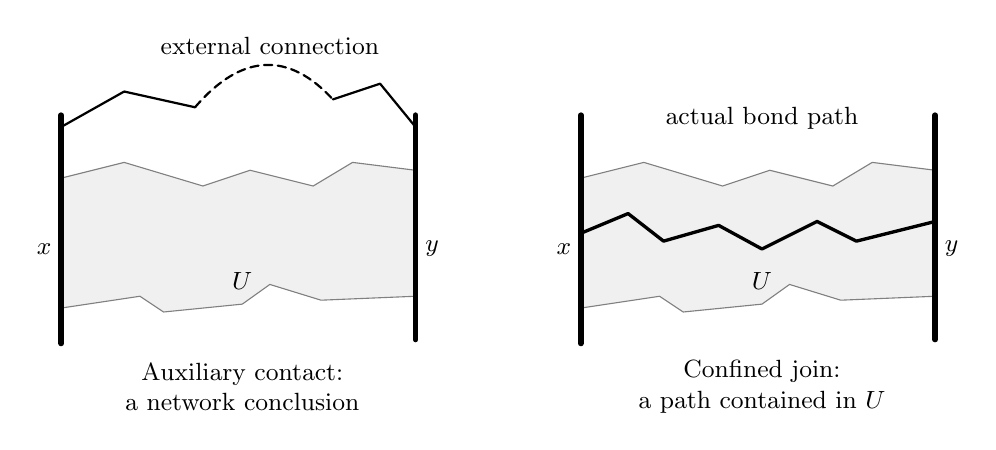
\begin{tikzpicture}[x=1cm,y=1cm,font=\small,line cap=round,line join=round]
  \foreach \shift in {0,6.6} {
    \begin{scope}[xshift=\shift cm]
      \path[fill=gray!12] (0,.75) -- (1,.9) -- (1.3,.7) -- (2.3,.8) -- (2.65,1.05)
        -- (3.3,.85) -- (4.5,.9) -- (4.5,2.5) -- (3.7,2.6) -- (3.2,2.3)
        -- (2.4,2.5) -- (1.8,2.3) -- (.8,2.6) -- (0,2.4) -- cycle;
      \draw[gray] (0,.75) -- (1,.9) -- (1.3,.7) -- (2.3,.8) -- (2.65,1.05)
        -- (3.3,.85) -- (4.5,.9);
      \draw[gray] (0,2.4) -- (.8,2.6) -- (1.8,2.3) -- (2.4,2.5) -- (3.2,2.3)
        -- (3.7,2.6) -- (4.5,2.5);
      \draw[line width=2pt] (0,.3) -- (0,3.2);
      \draw[line width=2pt] (4.5,.35) -- (4.5,3.2);
      \node[left] at (0,1.5) {$x$};
      \node[right] at (4.5,1.5) {$y$};
      \node at (2.3,1.1) {$U$};
    \end{scope}
  }
  \draw[thick] (0,3.05) -- (.8,3.5) -- (1.7,3.3);
  \draw[densely dashed,thick] (1.7,3.3) .. controls (2.3,4) and (2.9,4) .. (3.45,3.4);
  \draw[thick] (3.45,3.4) -- (4.05,3.6) -- (4.5,3.05);
  \node[above] at (2.65,3.85) {external connection};
  \node[align=center] at (2.3,-.25) {Auxiliary contact:\\a network conclusion};
  \draw[line width=1.2pt] (6.6,1.7) -- (7.2,1.95) -- (7.65,1.6) -- (8.35,1.8)
    -- (8.9,1.5) -- (9.6,1.85) -- (10.1,1.6) -- (11.1,1.85);
  \node[above] at (8.9,2.9) {actual bond path};
  \node[align=center] at (8.9,-.25) {Confined join:\\a path contained in $U$};
\end{tikzpicture}
\caption{Network contact and a confined join. The hubs $x,y$ represent
measured blockers or terminal walls, and $U$ is the untouched channel
between them. A network connection may use exterior graph portions
(left). Lemma~\ref{lem:confined-join} produces an actual open path
inside $U$ (right), under its separated-barrier, ordinary-incidence,
and planar-cap hypotheses. In a pure two-end-wire disk, network
connection already has an actual witness; the additional conclusion
here is confinement to the channel.}
\label{fig:actual-network}
\end{figure}


\subsection{Physical routing in regular geometries}

We next build prescribed physical connections from a finite chain of
crossing templates and confined joins. Free-wall attachments require
a separate seed construction. For several attachments, one further
point is essential: the local joins must belong to the same physical
component inside each shared corridor. The component estimate below
provides this compatibility before the final union bound.

All probabilities in this subsection are finite positive FK probabilities
at the fixed self-dual odds. A path called \emph{actual} uses open bonds,
including an ordinary terminal incidence when appropriate, and never
uses an identification as a path edge. Boundary incidences on different
banks of a slit remain distinct. Constants may depend on a fixed finite
collection of geometric shapes and their positive clearances. Geometric
parameters are fixed first; the mesh then tends to zero. In particular,
a positive lower bound for a fixed thin corridor need not remain positive
as its width tends to zero.

\begin{definition}[Regular collars and permitted exterior data]
\label{disk:regular-collars}
A regular radial collar is a full tile annulus or a union of a bounded
number of tile sectors separated by straight coordinate walls. The
sector angles belong to the fixed finite list of quadrant, half-plane,
three-quadrant, and slit geometries. Distinct banks and distinct corner
incidences are kept distinct. Tile-level cuts specify its two radial
sections. Designated wire intervals may run along the banks. Name every
identified bank class that meets the collar, whether it crosses the
whole collar or occupies only a partial bank interval, and suppose
their total number is at most a fixed $J$. These classes are the named
hubs of the collar; $J$ counts all of them, not just those meeting
both radial sections.

Exterior data are \emph{permitted} if they arise from finite FK graphs
with positive odds and have the following planar attachment structure.
The graph on either side meets the collar only at its own radial
section and the named hubs. It preserves all ordinary collar incidences
and designated wire portions, and has no other bank or interior
attachment. It may induce any partition on that section together with
the hubs, subject to the following residual-cap condition. In each of
the four quotients obtained by imposing neither, either, or both side
partitions, remove from the cap ledger every final class meeting a
named hub. The remaining classes must be separate noncrossing caps on
the two coordinated radial sections: place the sector strips side by
side in angular order and reverse the inner boundary order, resolving
coincident accesses in their separate fans. The two residual caps
occupy the two separate boundary arcs of this drawing.

When comparing two laws, the graph and deterministic wires on the
remote side agree; the other, unknown side may induce any permitted
partition. A rectangular bulk collar is an ordinary polygonal annulus
of fixed shape buffering a box, with positive relative width and no
internal wall. Local patches on a planar capped cylinder are permitted
only when the specified disk or sector charts satisfy this same
attachment and residual-cap contract.
\end{definition}

\begin{lemma}[The initial collar comparison]
\label{disk:initial-collars}
In the geometries of Definition~\ref{disk:regular-collars}, collars of a
sufficiently large fixed radius ratio give bounded reciprocal marginal
densities on their remote side, uniformly in the permitted unknown-side
data. The same holds in the opposite radial direction and for a fixed
rectangular bulk collar.
\end{lemma}

\begin{proof}
For a bulk collar this is Proposition~\ref{prop:annular-density}, with
polygonal cuts and ordinary buffers. For sectors, retain every named
bank class as a hub, including every partial bank interval. In each of
the four cross pressure masses entering the alternating
partition-function identity, discard terms hitting a final hub class.
Positive coverage and the singleton identity charge at most $J\log t$
for these terms, as in Lemma~\ref{lem:hub-mass}. All cap classes
absorbed into a hub are discarded with it. The residual-cap condition
in Definition~\ref{disk:regular-collars} supplies the separate
noncrossing caps on the coordinated cuts in each quotient. This is the
cap order needed by the clean comparison; the bound on $J$ alone would
not supply it.

Each complete clean sector is a tiled disk, and its blank actual radial
crossing probability is arbitrarily small at sufficiently large fixed
radius ratio, by Theorem~\ref{thm:actual-disk}. Their finite disjoint
union has the same property by a union bound. The separate-cap and
no-hit comparisons, followed by the alternating pressure identity,
therefore bound all four residual masses. This is precisely the sector
density argument, applied to the coordinated disjoint charts; adding
back the discarded hub terms leaves a uniform bound. The mixed
partition-function bound says that the relative weight of an exterior
state changes by a bounded factor when the opposite cap changes.
Summing over exterior states and normalizing proves the stated marginal
comparison. Reversing radial order makes the same proof apply inward.

If a chosen positive cap completion adds a fixed bounded number of
further block identifications, each changes every configuration weight
by either $1$ or $q^{-1}$, and these additions change normalized
densities by a bounded factor. Any additional bank class instead
retained in the collar must be included in $J$ and satisfy the same
attachment and residual-cap conditions. Thus the comparison does not
cover an unbounded collection of partial bank classes or unlisted
lateral attachments.
\end{proof}

\paragraph{Searches and their physical blockers.}
We use the physical face exploration of Lemma~\ref{sector:frontier}
in each tiled quadrilateral. Designate its end arcs as near and far,
and keep the longitudinal flank faces separate. Start from the
\emph{exterior} face of the chosen flank. An edge is queried only from
a reached complementary face; the opposite face is entered only if
the intervening tested-color physical bond is closed. In particular,
interior faces adjacent to the starting flank are not seeded for free.
The end cuts are impassable to this search. Fictitious exterior end
spokes specify only the disk separation topology: they are neither
physical path edges nor identifications in the FK law.

If an actual tested-color crossing exists, the search cannot reach
the other flank. Exhaust its reached component and temporarily set
the unqueried tested-color bonds closed. This does not enlarge the
reached component, since every edge leaving it has already been
queried and found open. The path/cut alternative therefore gives a
crossing supported on measured open bonds. Select the simple frontier
adjacent to the unsearched side by fixed tie breaks, orient it from
the near cut to the far cut, and retain the segment after its last
near-cut visit and before its first subsequent far-cut visit. Denote
this measured actual path by $P$. Its opposite-side edge interiors
and ordinary incidences remain unqueried. Temporary closure selects
the witness and imposes no additional condition on the random state.

One can require a crossing to be proper, meaning that it has no other
contact with its two end cuts. For this search, split the incidences at
an end vertex into separate leaves in fan order, ignore travel along
the end cut, and add fictitious outward terminal spokes. This changes
the search drawing, not the random states or the FK partition. A
simple trimmed physical witness gives the corresponding proper
crossing in this auxiliary drawing, even if it touches a longitudinal
wall or uses boundary bonds. At a shared wall incidence, an access
from the unsearched side meets the witness before or at that incidence.
All queries and physical paths remain in their original slot fans.
Known open diagonals serving as cutters have ordinary
half-tiles on their unqueried side; in the opposite color their new
boundary spokes are dangling or dead. Thus cutting at a measured
blocker gives free longitudinal boundary in that opposite color.

The shielding assertion is useful also in endpoint order. If a proper
witness ends before a specified opening in the far end cut, a search
from the witness's side cannot discover a frontier crossing ending
beyond that opening. Otherwise a reached complementary face incident
to its last bond could be continued inside that tile to the end cut
without meeting the witness. This contradicts separation by the
witness, which has no earlier contact with that cut. These statements
are statements in the split disk drawing, so they remain true with
boundary touches and coincident bank images.

Every successful orientation or endpoint-clearance alternative used
below is a union of leaves of its own deterministic edge exploration.
On an individual leaf, delete the queried closed edges and contract
the queried open components. Lemma~\ref{lem:finite-conditioning} gives
the exact FK law on the unqueried edges, with its induced planar
partition. Bounds on those leaves are averaged before conditioning on
any further success event. No FK law conditioned only on a union of
successful leaves is asserted.

\begin{proposition}[Actual routing and terminal attachments]
\label{prop:routing}
In a fixed regular patch with permitted planar exterior data, an actual
crossing of either color along a cleared simple corridor between two
short transverse cuts has probability bounded below by a positive
constant. The connection is confined to that corridor and small
prescribed endpoint neighborhoods. The conclusion is uniform when its
geometry has uniform positive clearances.

A terminal may instead be a continuous wire interval of the tested
color, an unwired flat wall interval, or a previously measured actual
blocker with a uniformly clear tangent-disk approach. In the last case
the blocker must be the only locally accessible obstruction from that
approach, allowing further portions of the same labeled barrier; its
ordinary unqueried incidences must be available up to the contacts.
An attachment to a measured blocker is an actual contact with that
path. An attachment to a wire requires just one actual wall contact.

Finitely many such attachments can be imposed simultaneously in the
following layouts: disjoint branch corridors arriving at spaced points
on a skinny joining tube; a four-terminal tree with two radial and two
wall branches; a ring of cleared corridors; or a corridor winding once
around a regular cylinder and returning to a distinct point of the
same joining tube. These conclusions hold conditionally on the
initial terminal exposures.
\end{proposition}

\begin{proof}
We prove the claims in an order that uses only the large-ratio collar
comparison already available.

\emph{Bulk templates and their gaps.}
The square-crossing and clipped-template construction in the proof of
the auxiliary contact lemma, Lemma~\ref{disk:auxiliary-contact}, supplies
the following finite collection of supports in a cleared corridor.
Small squares carry actual crossings between tiny selected subarcs of
two opposite sides, and clipped squares implement a right-angle bend.
Their individual conditional probabilities are positive uniformly in
planar exterior data. To recall why this is an actual-crossing input,
the square path/cut alternative gives probability at least $1/2$ for
one of a crossing and its complementary crossing. Duality, a grid
symmetry, and bounded ordinary annular marginal comparison transfer
the latter alternative to a crossing of the requested color. Splitting
the two end sides into finitely many short intervals selects endpoint
patches at a positive probability cost. Cropping a crossing gives the
clipped templates. Transfers and conditional lower bounds use ordinary
buffers around the whole support.

Here are the placement features that will be needed. Approximate the
cleared route by a simple axis-polygonal route at a fixed fine geometric
scale, erase loops, and keep positive clearance after this perturbation.
On a straight segment, pair a square template with its reflection so
that the two endpoint-center transverse displacements cancel. Adjust
the square side lengths to obtain the required axial advance. At a
right-angle turn use a square clipped by a transverse diagonal and a
reflected, traversal-reversed copy on the other side of that diagonal.
The entry and exit strips can be narrower than the bend supports, so
nonadjacent supports and their buffers are disjoint. Choose bend sizes
first. Their endpoint displacements are then fixed; two independent
axial segment adjustments absorb these displacements and all gap
lengths. This gives a fixed finite number of templates before the
final gap tolerances are chosen. Extend the first and last templates
across the desired corridor cuts and trim their crossings there.

Consecutive envelopes have tiny positive gaps between transverse end
caps and still smaller endpoint tolerances. On the event that every
template crosses, expose each extremal frontier from the same
longitudinal side of the oriented route. The exposures use disjoint
supports. Around the midpoint of a matching gap, and between radii
much larger than its width and much smaller than the template size,
the two measured blockers span an annulus in opposite open
half-planes. Their inward endpoints may be prolonged across the
innermost disk by fictitious spokes solely to specify their separation
topology. The blockers themselves are the barriers throughout the
annulus where the join lemma is applied.

The annular component on the unsearched side has no measured
incidence before it hits one of these blockers. Indeed an entry
through an envelope's unsearched flank is shielded by its frontier.
An entry through its searched flank is not in this component: that
flank has an exterior route to the other diameter ray without crossing
the blocker. At a straight cap this route goes around its lateral
edge. At a clipped bend, at the radii in question at most one lateral
corner intrudes; the cap and that side bound a wedge of fixed positive
angle, and one exits around its searched side. For a narrow normal
strip one exits around the corresponding parallel side. The two full
barrier spans separate the two rays, so none of these searched-side
entries is accessible from the focal component. This also excludes
folded measured bays. Bounded tile-rounding errors are absorbed in
the strict half-plane margins and a fixed enlargement of the radial
band. These are the hypotheses of Lemma~\ref{lem:confined-join}.

Let $S$ be the intersection of the template successes. Their disjoint
buffer estimates give $\PP(S)>0$. The successful leaves already
determine $S$. On every such leaf the probability of failure of any
specified actual join tends to zero as the gap ratio tends to infinity,
uniformly in the permitted remaining data. A finite union bound thus
joins the entire chain with positive conditional probability. Each
join is physical and confined to its prescribed patch. This proves
bulk corridor crossing without making any connection through an
external wire.

\emph{A wire or a measured tangent blocker.}
For a straight wire interval, terminate a thin bulk strip at a small
positive normal distance from the wall and expose its frontier on a
compatible side. The wall and this blocker are the two barriers for
the same confined-join argument. The resulting actual path stops at
one contact of the specified wire.

More generally let a tangent disk of radius $c'>0$ touch the measured
blocker at $z$, with the stated ordinary cleared approach. Terminate
the incoming branch at distance $\epsilon$ along the inward normal,
using a still thinner straight normal strip in a patch of radius $s'$.
Choose
\begin{equation}\label{disk:tangent-scales}
       (s')^2/c'\ll\epsilon\ll s'\ll c'.
\end{equation}
In coordinates tangent at $z$, disk exclusion confines every accessible
part of the old blocker to a half-plane enlarged by
$O((s')^2/c')$. The incoming strip is on the other side of the middle
diameter with margin of order $\epsilon$. Between an inner radius
larger than the gap and an outer radius smaller than $s'$, both
barriers span the annulus in opposite half-planes. Only the specified
blocker label is accessible at the old wall. Applying the confined
join therefore makes an actual attachment to the measured path, with
failure arbitrarily small. The hierarchy in
\eqref{disk:tangent-scales} is chosen before the mesh limit. Cleared
routes and tangent normals in a compact family admit uniform choices,
by a finite pixel approximation of their interior routes, or by taking
a position limit and retaining strict sub-clearances.

\emph{A free-wall seed.}
Consider first a blank tested-color law in a flat half-box. A small
central wall interval has positive probability of an actual arm to
the opposite line. To see this, separately wire that interval and
the opposite line. Lemma~\ref{disk:auxiliary-contact} gives a positive
two-terminal probability. With only these two wires, network
connection is equivalent to an actual path between the two sets:
erase all visits to an end wire before the last departure and after
the first arrival. The no-hit comparison of Lemma~\ref{lem:no-hit}
makes the blank actual probability at least this pure probability.
Denote a resulting lower bound by $p_0>0$.

Put a protected wall rectangle around the central interval, with a
fixed positive lateral margin $a$. An arm going to the opposite line
either reaches height $\eta$ within that rectangle or exits it
laterally while staying below height $\eta$. Choose many disjoint
boxes of dimensions comparable to $\eta$ along either possible
lateral exit route. In each, the opposite color, which is wired on
this wall, has an actual transverse arm from the wall to above height
$\eta$ with conditional probability at least $c_1>0$. This is the
already proved wired-wall construction in a fixed shape. These arms
block the tested-color lateral excursion. With at least
$c_2a/\eta-O(1)$ tests, its probability is at most
\[
  2(1-c_1)^{c_2a/\eta-O(1)}.
\]
Choose $\eta>0$ so this is less than $p_0/2$. The protected actual
wall-to-height event then has probability at least $p_0/2$.

Choose the wall-seed scales small compared with the available straight
wall patch. The protected rectangle can then be surrounded by a
half-sector collar of the sufficiently large fixed ratio in
Lemma~\ref{disk:initial-collars}, inside the original flat patch. This
transfers its positive probability to every permitted exterior with
the same free tested-color wall. Expose an extremal seed inside its
protected rectangle, stopping at a fixed height below the height just
obtained. The region above that cut is untouched. Its endpoint
determines an incoming approach from that region; the branch is
chosen after observing the seed. At the much smaller attachment scale
the cut is a straight transverse cap, including the one-corner wedge
case if the endpoint lies at a lateral corner. Choosing the compatible
exposed side of the incoming branch gives the gap geometry already
checked. A confined join attaches to the physical seed, which in turn
is physically connected to the unwired wall. Notice that this argument
has used large-ratio sector comparison only. Thin-ratio comparison
will be deduced after the physical screens have been constructed.

\emph{Traversals in one physical component.}
Two attachment searches can select different traversals of the same
corridor. We therefore need the following claim before combining the
attachments. Let $C$ be a branch corridor or joining tube with whole
end cuts $A_C,B_C$, let $E_C$ be its actual traversal event, and let
$U_C$ be the event that all its proper actual traversals lie in one
physical component supported in $C$. Put
\[
 \alpha_C=
 \frac{1+\max\{\operatorname{diam} A_C,
                    \operatorname{diam} B_C\}}
      {\operatorname{dist}(A_C,B_C)},
\]
with lengths in tile units. The claim is
\[
 \PP(U_C^c\cap E_C)\le o(1)\PP(E_C)
 \qquad\text{as }\alpha_C\longrightarrow0,
\]
uniformly in permitted exterior data, including fixed states in
disjoint supports. Narrow end cuts and then fine mesh make
$\alpha_C$ small in our fixed layout.

To prove the claim, expose the two extreme frontiers toward the
middle. Their successful leaves determine $E_C$. Every other
traversal disconnected from them must
lie between them, since a traversal farther toward either searched
side would shield the corresponding measured frontier from that
search. If the frontiers are disjoint, the disk between them has
unqueried interior and free opposite-color longitudinal flanks. Its
possible extra identifications are planar joint end caps. Failure of
an actual join between the frontiers in this disk forces an actual
opposite-color traversal between its end arcs. The latter has
probability $o(1)$, uniformly on these leaves, by
Theorem~\ref{thm:actual-disk}, because its two ends are subarcs of
$A_C,B_C$ and have separation ratio tending to infinity with
$\alpha_C^{-1}$. A transverse actual join intersects
every proper traversal between the two frontiers. If the frontiers
intersect, shielding already excludes a traversal disconnected from
both. Boundary contacts are separated in their own fans; the
half-tile convention along a known open cutter makes precisely the
free opposite-color boundary used in this application. The failure
bound holds on each successful pair of frontier leaves. Averaging
those leaves proves the displayed relative estimate.

\emph{Simultaneous attachments.}
Place a long skinny joining tube of half-width $w$ in the clear middle.
Draw nonintersecting buffered branch corridors to spaced points along
its length. Near a top arrival a branch stays above transverse
coordinate $2w$ and ends in a thin normal strip; bottom arrivals are
reflected. Their distant ends have the already specified terminal
geometry. All corridor and tube success events have jointly positive
probability by successive conditional lower bounds. Denote their
intersection again by $S$. We will bound physical failures conditional
on $S$ by first obtaining uniform bounds on exploration leaves that
decide $S$ while leaving the relevant join region unqueried.

For corridor $j$ let $U_j$ be the physical event that all its proper
traversals belong to one component within it. For attachment $i$ let
$J_i$ be the physical event that a local path joins some successful
traversal in each of its two incident supports, or attaches one such
traversal to the indicated terminal blocker or wall contact. To bound
$J_i^c$, explore just the pertinent frontiers from the sides suitable
for that attachment and fix the other disjoint support states away
from its patch. The fixed outside states decide the successes of the
other supports; the frontier leaves decide those of the two incident
supports. Thus each retained combined record decides $S$, and its
unqueried join region has the ordinary conditional FK law. At a top
tube arrival, search the tube from its bottom lip.
Its whole frontier is below height $w$. Center the separating
horizontal diameter in the gap above it; both focal directions above
the tube are available, and select the one exposed by the branch
search. The tube has two continuations with its same label, as allowed
in Lemma~\ref{lem:confined-join}. The previous cap and tangent arguments
handle the other terminals. Hence for any prescribed $\varepsilon>0$
the fixed geometries can be chosen so that the failure bound is at
most $\varepsilon$ on every retained record. The component claim
gives the same conclusion for $U_j^c$ by using that corridor's two
frontiers and fixing the other supports. Averaging each experiment
separately gives
\[
 \PP(J_i^c\cap S)\le\varepsilon\PP(S),\qquad
 \PP(U_j^c\cap S)\le\varepsilon\PP(S),
\]
and hence
\begin{equation}\label{disk:conditional-joins}
 \PP(J_i^c\mid S)\le\varepsilon,\qquad
 \PP(U_j^c\mid S)\le\varepsilon.
\end{equation}
For $k$ attachments and $m$ corridors it follows that
\begin{equation}\label{disk:physical-union-bound}
 \PP\left(\bigcap_{i=1}^k J_i\cap
                 \bigcap_{j=1}^m U_j\,\middle|\,S\right)
       \ge 1-(k+m)\varepsilon.
\end{equation}
On this event all the selected attachments belong to the intended
physical components. Different attachments may require different
orientations of the same exploration: the estimates are for the
physical events $J_i$, so their explorations need not coexist. The
error bound remains $\varepsilon$ even when $\PP(S)$ is small.

For clarity, choose the fixed finite layout and its mutual clearances
first, then the join patches and required radial ratios, then the
narrow strip and endpoint tolerances, and finally the mesh. At a
tangent terminal shrink its patch further to satisfy
\eqref{disk:tangent-scales}. With
$\varepsilon<1/(2(k+m))$, \eqref{disk:physical-union-bound} proves
the desired positive probability. All its paths use just the corridors,
their small join neighborhoods, and the measured terminal blockers.

A four-terminal tree is obtained by two opposite-side wall branches
at spaced central tube positions and two radial branches at its
longitudinal portions. A ring uses a finite cyclic chain of corridors.
On a cylinder choose a simple winding corridor with separated ends
at two distinct tube positions. Its actual traversal, joined at both
ends to the connected tube, gives a closed walk with nonzero winding
number: the tube return lies in a disk and the corridor winds once.
Deleting contractible loops from that walk leaves a noncontractible
actual cycle. This finishes all the asserted layouts.
\end{proof}

\begin{proposition}[Actual screens]
\label{prop:screens}
For each fixed regular collar geometry, either color has an actual
wall-to-wall screen in a sector, or an actual surrounding circuit in
a full annulus, with a uniformly positive conditional probability
under permitted exterior data. The paths remain in a prescribed
middle subcollar and meet every designated continuous through wire
of the tested color when those are present. The statement includes straight walls,
quadrant and reentrant corners, slit tips, and differing wire
designations on the banks near a flip. Contacts are chosen on
straight bank patches separated from the tip or corner apex.
Different colors in tile-disjoint sectors can be required together.
\end{proposition}

\begin{proof}
Choose bank patches away from the finitely many apexes and draw a
cleared transverse route in each sector. Use a wire contact or a
free-wall seed according to the color designated on that bank.
Proposition~\ref{prop:routing} constructs the entire actual screen.
For an annulus, use the ring layout around its inner boundary; its
closed actual walk contains a surrounding simple circuit. For a
finite collection of disjoint sectors impose the specified screens
successively, conditioning on the other support states; each retained
law still has the permitted planar exterior data. The product of
the finitely many positive lower bounds is positive. Distinct slit
banks are treated in their own charts, so physical coincidence does
not join their incidences. No path in this construction uses a wire
as an edge.
\end{proof}

\begin{lemma}[Fixed-ratio sector comparison]
\label{disk:thin-collars}
Lemma~\ref{disk:initial-collars} holds also for a fixed smaller
nontrivial sector ratio, with a constant depending on that ratio and
the fixed geometry.
\end{lemma}

\begin{proof}
First consider the clean disjoint union of sectors, without bank
hubs. In its blank tested-color law, an actual opposite-color screen
in each component blocks radial traversal. Under duality the opposite
color has the requisite wired wall conditions, and
Proposition~\ref{prop:screens} applies conditionally. Thus the blank
actual radial probability $b$ satisfies $b\le1-\eta_0$ for some
$\eta_0>0$.

The blank cross pressure mass $\Delta$ is bounded as well. Cover one
radial cut by finitely many small interval patches, of diameter tiny
compared with the collar depth. For a patch in one component the
pure connection probability to the other entire cut is arbitrarily
small by Theorem~\ref{thm:pure-disk}; all other components attach
only to the latter full wire and do not change this test. The
one-sided density estimate bounds the pressure mass for this pair.
Positive coverage and the finite patch cover bound $\Delta$ for
the full two cuts. The cofacial one-sided comparison gives the
corresponding bound after either single cap is imposed.

Write $Z_{ab}$ for the four cap choices, and $\Delta_{ab}$ for
their cross masses. The alternating identity reads
\[
 \log\frac{Z_{11}Z_{00}}{Z_{10}Z_{01}}
       =\Delta_{10}+\Delta_{01}-\Delta_{00}-\Delta_{11}.
\]
The blank no-hit mixed-gain bound, using $b\le1-\eta_0$, supplies
a lower bound for the logarithm. Nonnegativity and the three bounds
just proved therefore bound $\Delta_{11}$ and the mixed logarithm
in both directions. This proves bounded reciprocal densities for
the clean union. Discarding all at most $J$ named bank-hub
classes and retaining the coordinated residual noncrossing caps,
exactly as in Lemma~\ref{disk:initial-collars}, proves the general
statement. The proof uses the physical screens only here, after
their construction; the wall seeds used only the earlier large-ratio
comparison.
\end{proof}

\subsection{Relative localization through restricted collars}

Bounded density comparison preserves a positive probability but does
not make distant boundary data negligible. A screen that meets every
possible through wire removes that dependence altogether on a fixed
positive part of the collar law. Repeating this common part, and
retaining one final bounded comparison, gives a relative error for
every nonnegative observable, including rare events.

\begin{proposition}[Relative collar comparison]
\label{prop:relative-collars}
Consider two finite positive FK laws at the fixed $q$, with ordinary
collar bonds, whose graphs and deterministic wires agree on the remote
side of a sequence of regular collars and whose unknown-side data are permitted in the sense of
Definition~\ref{disk:regular-collars}. Require each collar to have
one of the following geometries:
\begin{enumerate}[label=(\roman*)]
\item a full annulus with no named bank hubs, or one sector whose only
bank attachments are continuous primal wire portions along its two
side rays, crossing the collar and each met by its primal
wall-to-wall screen;
\item two sectors, with only such screen-met continuous primal wire
portions on both side rays of one sector, no bank or hub attachment in
the other, and no direct contact between the sectors inside the collar.
Side graphs may join contacts of the two sectors only through the
corresponding permitted radial cap.
\end{enumerate}
After $m$ further collars of a sufficiently large fixed ratio and
one final comparison collar, the expectations of any fixed
nonnegative function $f$ supported beyond them satisfy, for fixed
$C\ge1$ and $0<c<1$, the two inequalities
\begin{equation}\label{disk:relative-density}
 \begin{split}
 \EE_1 f&\le\bigl[1+(C-1)(1-c)^m\bigr]\EE_2 f,\\
 \EE_2 f&\le\bigl[1+(C-1)(1-c)^m\bigr]\EE_1 f.
 \end{split}
\end{equation}
They are understood in the extended nonnegative reals. For finite
positive expectations they imply
$\EE_1 f/\EE_2 f=1+O((1-c)^m)$, and the expectations vanish together.
The constants are independent of the far graph, the unknown-side
partition, and $f$. The same conclusion holds in the reverse radial
direction and after a positive finite tilt supported on the unknown
side. In particular, unknown-side changes may join or separate the
designated wire portions. The contraction requires the enumerated
screen-met attachments; the general bound on $J$ in
Definition~\ref{disk:regular-collars} alone is not sufficient for it.
\end{proposition}

\begin{proof}
We give the finite FK comparison and coupling argument. It also explains
the restrictions on the geometry. Throughout a comparison, keep the
entire common graph beyond the current section fixed, including its
far boundary data. Collar marginals can depend on this remote graph;
all constants below are uniform in that dependence.

Split each designated wire transversely
at a section, retaining its connections separately on either side
and one representative of the possible through connection. There
are only boundedly many such representatives. The unknown graph
then enters the common graph as a permitted partition $\xi$ on that
section, with all the common deterministic wire pieces included.
Any bounded extra split or merger has weight ratio between
$\min(q,q^{-1})$ and $\max(q,q^{-1})$ per operation. The bounded
collar comparison therefore applies equally to this representation.

Use a sufficiently large fixed ratio, for example enlarge a factor
$256$ further if needed, to leave two buffered subcollars at every
step. Fix a reference permitted partition. The initial comparison
subcollar makes the marginal $\mu_\xi$ on the second subcollar
dominate $K^{-1}\mu_*$ for every $\xi$, with a constant $K$ and
the same reference marginal $\mu_*$. This is a pointwise inequality
of finite measures on the subcollar edge configurations.

Inside that second subcollar, in case (i) require a primal circuit,
or a primal wall-to-wall screen meeting every named primal bank wire.
In case (ii) require a primal screen in the wired sector and a dual
screen in the other. Proposition~\ref{prop:screens} gives a reference
probability at least $p_*>0$ for this event $G$. On $G$, the partition
transmitted to the next section is determined by the common
subcollar configuration alone. Indeed every connection from the
unknown side to the remote side in a screened primal component must
meet a connected primal screen. All named bank wires there
already meet that same screen. Connections through the unknown
region can therefore make no further distinction among its remote
contacts. In the unwired second sector the dual screen allows no
actual primal crossing, and there is no bank or hub attachment to bypass it.
The absence of other intersector contacts is used at exactly this
point.

Any cluster of the common subcollar meeting the next section but
avoiding the transmitting screen is therefore unable to acquire
an extra connection through the unknown region. Components wholly
on the exposed side contribute factors independent of all remote
states and cancel when the conditional law is normalized. By the
finite domain Markov identity, the entire conditional remote law
thus depends only on this transmitted partition.

For completeness, screens can be discovered without querying edges
strictly beyond them. Explore complementary-color components from
the unknown-facing section. If the screen exists, the search stops
short of the remote section; otherwise the disk path/cut alternative,
or its annular version, would give a complementary crossing. The
measured frontier consequently contains a blocking physical path or
circuit. Perform this search in the buffered middle and reverse
colors in the unwired sector. Thus the same transmitted-partition
description applies either by revealing the whole fixed subcollar
or by stopping at its measured screens.

To specify the transition precisely, reveal the tile states up to the
next section and let $\eta$ be the partition they induce there from
the exposed side, together with the common deterministic wire pieces.
The planar drawing and the absence of unlisted lateral attachments
keep $\eta$ in the permitted class. Conditional on the exposed states,
the law of the fixed remote graph is the FK law with partition $\eta$,
by Lemma~\ref{lem:finite-conditioning}. Thus, for a remote observable
$f$, its conditional expectation is a function $g(\eta)$ of that
partition. On the screen event $G$, the preceding separation argument
shows that $\eta$ is determined by the second subcollar configuration
alone and is independent of the entering partition $\xi$. Away from
$G$ it may also depend on the first subcollar and on $\xi$.

The measure
\[
        \lambda=K^{-1}\one_G\mu_*
\]
is a common submeasure of all second-subcollar laws and has mass at
least $p_*/K$. On its support the just-defined map to $\eta$ is common
to all entering partitions. Its pushforward is therefore a common
submeasure $\nu$ of the laws $L_\xi$ of the induced next partition,
with the remote graph still held fixed. These laws are the transition
kernels used below. Choose a fixed $c>0$ not exceeding
$p_*/K$, and reduce $\nu$ to mass $c$ if necessary. Every such
kernel has the form
\begin{equation}\label{disk:collar-minorization}
       L_\xi=c\widehat\nu+(1-c)\widetilde L_\xi,
\end{equation}
where $\widehat\nu$ is the same probability measure for all
$\xi$. This is the common positive part of a coupling. No
stochastic monotonicity of FK boundary conditions is required.

For a bounded nonnegative $f$, make the relative-error deduction explicit.
Number the sections
$0,1,\ldots,m$ toward the support of $f$ and reserve the final
bounded-comparison collar beyond section $m$. Let
$[a_j,b_j]$ be the range of conditional expectations of $f$ over
all permitted partitions at section $j$, including the common
remaining graph. Conditioning on the next section gives
\[
 [a_j,b_j]\subseteq[a_{j+1},b_{j+1}],\qquad
 b_j-a_j\le(1-c)(b_{j+1}-a_{j+1}),
\]
where the second assertion follows from
\eqref{disk:collar-minorization}. The last comparison collar gives
$b_m\le C a_m$. If $a_m=0$, then $b_m=0$ and all expectations
vanish. Otherwise $a_0\ge a_m>0$ and
\[
 \frac{b_0-a_0}{a_0}
 \le (1-c)^m\frac{b_m-a_m}{a_m}
 \le (C-1)(1-c)^m.
\]
It follows that either expectation is at most
$[1+(C-1)(1-c)^m]$ times the other. This proves
\eqref{disk:relative-density} for bounded $f$. For a general
nonnegative $f$, apply those two inequalities to $f\wedge M$ and let
$M$ increase by monotone convergence. No quotient of infinite
expectations is used.

The same proof works inward, using the reversed collar comparison
and the same separation by actual screens. A positive modification
on the unknown side merely changes the mixture over its induced
partitions: every member has the same common submeasure and lies
in the same interval $[a_0,b_0]$. Integration over that mixture
proves the assertion about tilts. In particular no fixed connection
through a gap has to be retained when the gap belongs to the unknown
region. In case (ii) this is why both colors of screen, rather than
only the screen meeting the primal wires, are required.
\end{proof}

\subsection{Relative arm splices and an opposite-arm loss}

The remaining construction preserves a specified arm event while
joining its truncated pieces through a fresh window. Its probability
must be compared with that of the original arm, which may be very
small. A finite cover by one-sided exploration successes supplies this
relative comparison; the reconstruction also inserts a transverse
screen when an opposite-color radial arm must be excluded.

\begin{lemma}[A flat splice and strict opposite-arm cost]
\label{lem:relative-arm}
Let $A$ require an actual radial traversal of a specified color in a
long regular half-annular region whose two longitudinal walls carry
the continuous portions of a flat mixed-color boundary condition.
The start is a full inner cut or a specified flip-gap vertex and
the target is a full outer cut. Choose mutually separated marker
bands, with broad fixed-proportion splice windows on both sides of
each marker. Let $B_i$ require an actual opposite-color radial
traversal of marker $i$. There is $c>0$, depending only on the fixed
window shapes, such that
\begin{equation}\label{disk:opposite-arm-loss}
 \PP\left(A\cap\bigcap_{i=1}^k B_i\cap E\right)
 \le (1-c)^k\PP(A\cap E)
\end{equation}
whenever the extra requirement $E$ is supported outside those
windows. The estimate is uniform under permitted exterior
conditioning. A separated short arm can be included in $E$.

For the splice conclusion, let $T$ be the joint event of two
same-color actual arms, each supported in one of the two disjoint
side domains from its prescribed source to a full cut on its side
of a fixed-ratio window. Assume the same regular half-annular
geometry and fixed positive buffers as above, with two spaced
openings away from the flanks on each cut. Each source lies on the
opposite radial end of its side domain; a flip-gap tip is allowed
as an inner end. In units of the window scale, the distance from
the source to its window-facing cut is bounded below by a fixed
positive constant, and a side band of fixed positive depth adjoining
that cut is free of previously fixed far data. If $A_{\mathrm{join}}$
is the event that these sources are joined by an actual path in
the union of the side domains and the window, then
$\PP(A_{\mathrm{join}})\ge c\PP(T)$, uniformly under permitted
exterior conditioning. A single arm can be extended through
a further fixed-factor collar with a fixed relative probability.
Iteration gives polynomial arm lower bounds in these regular
geometries, and opposite-color screens give a strict power upper
bound for one-arm probabilities.
\end{lemma}

\begin{proof}
Fix one marker, write $B$ for its opposite-color traversal, and
condition on the edge states $F$ outside its broad window. Other
marker constraints and $E$ are thereby decided. Trim any witness
for $A$ at two cuts lying just inside the window on its respective
sides of the central marker. It gives actual paths from the two
required sources to these cuts in disjoint side domains. A source
can include a previously measured physical continuation through
$F$, but no search follows a wire identification as a path edge.

At each near cut choose two small, spaced opening intervals away
from the flanks and corners. Orient each witness toward its target
cut and retain the portion after its last source-set visit and before
its first subsequent target-cut visit. Every resulting endpoint is
a fixed positive distance to one side of at least one opening.
Run a complementary search from that endpoint's side, treating
previously fixed far states as known data. The shielding argument
given before Proposition~\ref{prop:routing} makes its measured
frontier end on the same side of the selected opening. In
particular that opening is on its unqueried side with a uniform
margin. There are only a bounded number of choices of opening and
orientation at each end. Let $T_1,\ldots,T_N$ be the corresponding
two-search success alternatives. They satisfy
\begin{equation}\label{disk:truncated-cover}
       A\subseteq\bigcup_{i=1}^N T_i
\end{equation}
for each fixed $F$, with $N$ independent of mesh and scale. On each
successful leaf retain the simple actual frontier $P$ connected
physically back to its required source. Each $T_i$ is a union of leaves
of its own pair of searches, performed in the two disjoint side
domains. The uninspected regions have their usual conditional FK laws
on individual leaves; we do not condition those laws on the union in
\eqref{disk:truncated-cover}.

We verify the uniform tangent access needed to reconstruct between
the two frontiers. From the empty central region enter a chosen
opening, then move a small fixed radial distance into its side
band and along a level transversal toward the searched flank.
This route must meet $P$: the source-to-cut crosscut separates the
opening side from that flank. Start at a fixed clear point in the
central region, and choose a clearing radius $a$ smaller than its
boundary distance, the opening separation, and all side-band margins.
Move a center from that point along the route until its first distance-$a$
approach to $P$. The resulting disk is empty and tangent to $P$.
On entering the opening its endpoint is excluded by the angular
margin; along the transverse portion it is excluded by the radial
depth. Both cuts, all fixed far data, and the other flank stay at
larger fixed distances. Any approachable point of the searched
flank is screened by $P$, or is itself a contact with $P$. Hence
there is no other locally accessible wall before the tangent
contact. The unqueried incidences up to it are ordinary. Both endpoints
of $P$ lie outside a fixed enlargement of the contact neighborhood by
the cut margins, so both branches of $P$ continue out of it. Folds behind $P$
do not affect this disk. Tile rounding is absorbed by decreasing
the chosen fixed margins. This verifies all the measured-terminal
hypotheses of Proposition~\ref{prop:routing}, uniformly in the
successful leaves. Perform the same construction at the other end.

In the clear center of the marker put a skinny tube. Two separated
branches go to the tangent approaches just obtained; two further
branches go to the two walls, with their attachment sites spaced
on opposite tube sides. Use a wired contact or the free-wall seed
as required by each wall's tested-color designation. Seed
rectangles are disjoint protected patches, exposed first. The
radial branch detours remain in their respective radial
neighborhoods, while the wall-to-wall portion remains wholly
inside the marker. The four-terminal layout of
Proposition~\ref{prop:routing} consequently has a uniform positive
conditional probability $c_0$ on every successful leaf. It both
joins the two physically source-connected frontiers, preserving
$A$, and contains a same-color wall-to-wall screen inside the
marker. The screen excludes $B$ by planar path/cut separation.

Here is the relative, rather than merely absolute, estimate.
Integration over the leaves of any fixed alternative gives
\begin{equation}\label{disk:relative-reconstruction}
 \PP(A\cap B^c\mid F)\ge c_0\PP(T_i\mid F)
       \qquad(1\le i\le N).
\end{equation}
Take the largest of these right sides and use
\eqref{disk:truncated-cover}. It follows that
\[
 \PP(A\cap B^c\mid F)
       \ge\frac{c_0}{N}\PP(A\mid F),\qquad
 \PP(A\cap B\mid F)
       \le\left(1-\frac{c_0}{N}\right)\PP(A\mid F).
\]
Thus truncated success is used as an upper cover of the original
arm event; it need not already imply that event. Averaging in $F$
while retaining the exterior requirements and iterating over the
separated windows proves \eqref{disk:opposite-arm-loss} with
$c=c_0/N$.

For the two-arm event $T$ in the statement, use the same
opening and tangent constructions and join their two radial
branches in the clear middle. No transverse screen is required.
The two-success alternatives cover the separately required arms,
and the identical bounded-union calculation gives the fixed
relative probability. For extension of a single arm use one
truncated search and one new outer terminal. The constants are
uniform in the fixed rescaled geometry. Starting at a bounded
number of mesh steps, a specified finite physical path has a
positive conditional probability depending only on that bound
and the fixed $q$. Multiplying a fixed positive extension factor
over $O(\log(R/r))$ collars gives a polynomial lower bound.
For an upper bound, separated fixed-ratio bands have conditional
probability bounded below of an actual opposite-color screen by
Proposition~\ref{prop:screens}. An actual arm avoids every such
screen. There are at least $a\log(R/r)-b$ tests for fixed $a>0$ and
$b<\infty$, so successive conditioning gives an upper bound
$(1-c')^{a\log(R/r)-b}\le C(r/R)^{c''}$ for some $c''>0$.
These estimates require no independence
of the successive bands.
\end{proof}

The cylinder application keeps a short arm near a boundary mark and
a separate long arm farther out. Small conditioned endpoint boxes
lie in the gap between them. Comparing this joint two-piece event
across the boxes' buffers avoids conditioning on a rare completed
arm. A fresh splice then crosses the gap and attaches the arm to a
winding cycle. The opposite-color marker windows are placed along
the long piece, away from all conditioned boxes and both splice
constructions.

\begin{corollary}[The grouped cylinder splice]
\label{disk:grouped-cylinder}
Let $\mathcal C$ be a finite tiled cylinder of circumference comparable
to $n$, with finite positive FK cap graphs drawn planarly at its rims.
Its bottom has a flat mixed-color boundary near a specified flip-gap
vertex $s$, and a second marked bottom point $t$ at distance comparable
to $n$. All tiles in the following charts are ordinary. Fix their shape
and buffer constants first, then take $n/r$ sufficiently large and
$r$ sufficiently large in tile units.

There are finitely many endpoint boxes in the bulk near $s$, with
distances from $s$, depths from the bottom, and mutual spacings between
fixed positive multiples of $r$. Their radii are at most $\delta r$,
where $\delta>0$ is fixed sufficiently small. Each box has a disjoint
ordinary bulk-annular buffer, of fixed relative width, within the
scale-$r$ half-disk. Choose $c_0>0$ and $C_0<\infty$ so that these
buffers lie strictly between radii $c_0r$ and $C_0r$ about $s$, with
fixed positive margins. Their complement in this gap contains the
clear two-arm splice layout of Lemma~\ref{lem:relative-arm}.

Choose fixed $0<c_1<c_2$ so that the $s$-centered half-disk of radius
$c_2n$ is an injective flat cylinder chart. The half-sector collar
between its tile-level cuts at $c_1n$ and $c_2n$ has a sufficiently
large fixed ratio for Lemma~\ref{disk:initial-collars}. The $t$ box,
of radius at most $\delta n$, and the remote middle region lie outside
the $c_2n$ chart with positive $n$-scale margins. The attached graphs
at this chart and at every endpoint buffer satisfy
Definition~\ref{disk:regular-collars}, with a fixed bound on all named
bank classes and its residual-cap condition. In particular the graph
outside the $s$ chart attaches only at its outer radial cut and those
named hubs. A regular bulk window before the $t$ box and the middle
contains a joining tube and a cleared corridor winding once between
two distinct tube positions, as in Proposition~\ref{prop:routing}.
For each of two spaced flat openings on the $c_1n$ target cut, a
cleared branch joins its outward ordinary neighborhood to the tube.
The branch and winding buffers have fixed positive $n$-scale
clearances from the conditioned regions and satisfy the permitted
local-chart contract.

Let $\mathcal D$ specify the edge states in the endpoint boxes, the
$t$ box, and the remote middle; consider any feasible value of these
data. Let $R_{\mathrm{arm}}$ be the intersection of a short actual
gap arm from $s$ to radius $c_0r$ and a separate same-color actual
radial traversal from radius $C_0r$ to radius $c_1n$, both in the
flat half-disk chart. Their supports avoid all the endpoint buffers.
Choose a finite positive FK reference cap law that agrees with the
cylinder law on the graph, odds, and deterministic wall portions
through radius $c_2n$, including the endpoint buffers, and whose
exterior at that cut is permitted. Let $A_{\mathrm{ref}}$ be its full
actual gap arm from $s$ to a fixed full cutoff of radius comparable
to $n$ and strictly beyond $c_1n$, with a fixed buffer. Put
\[
 p_{\mathrm{ref}}:=\PP_{\mathrm{ref}}(A_{\mathrm{ref}}).
\]
The cutoff separates $s$ from the outer continuation of the reference
chart, so trimming gives $A_{\mathrm{ref}}\subseteq R_{\mathrm{arm}}$.
Let $E$ require an actual arm from $s$ joined to a noncontractible
actual cycle in the stated bulk window. There is $c>0$ such that
\begin{equation}\label{disk:grouped-cycle-lower}
 \PP(E\mid\mathcal D)
    \ge c\PP(R_{\mathrm{arm}}\mid\mathcal D)
    \ge c^2 p_{\mathrm{ref}}.
\end{equation}
For $k$ mutually separated opposite-color marker-traversal
requirements $B_1,\ldots,B_k$, with their full splice windows
between radii $2C_0r$ and $c_1n/2$, one also has
\begin{equation}\label{disk:grouped-marker-upper}
 \PP\left(R_{\mathrm{arm}}\cap
                  \bigcap_{j=1}^k B_j\,\middle|\,\mathcal D\right)
 \le C(1-c)^k\PP(R_{\mathrm{arm}}\mid\mathcal D).
\end{equation}
Here $C=1$ is possible when every listed marker has its full
window; the constant permits omission of boundedly many end
markers. The constants depend on the fixed buffer choices and
reference cutoff, but not on $r,n,k$ or the values of $\mathcal D$.
\end{corollary}

\begin{proof}
Write $\mathcal D_{\mathrm{out}}$ for just the $t$-box and middle data.
First remove the conditioning in the endpoint boxes one at a time.
Each disjoint bulk-annular buffer separates that box from the entire
support of $\one_{R_{\mathrm{arm}}}$. The inward or outward bounded
comparison of Lemma~\ref{disk:initial-collars}, while holding all
other data fixed, compares a specified box state with the mixture over
its states. The number of boxes is fixed, so
\[
 \PP(R_{\mathrm{arm}}\mid\mathcal D)
 \ge c_0'\PP(R_{\mathrm{arm}}\mid\mathcal D_{\mathrm{out}}).
\]
Next apply that lemma inward across the $s$-centered half-sector
between $c_1n$ and $c_2n$. The remaining cylinder law and the
reference law agree on its inner side, including the now unconditioned
endpoint boxes. The $t$ and middle states change only its permitted
outer partition, with every bank class included in the named bound.
Consequently
\[
 \PP(R_{\mathrm{arm}}\mid\mathcal D)
   \ge c\PP_{\mathrm{ref}}(R_{\mathrm{arm}})
   \ge c\PP_{\mathrm{ref}}(A_{\mathrm{ref}})=c p_{\mathrm{ref}}.
\]
Both comparisons use the single joint observable
$\one_{R_{\mathrm{arm}}}$. In the fixed-ratio gap about scale $r$,
these requirements force the
two truncated successes used in the splice proof. The finitely
many small separated endpoint patches can be avoided by disjoint
interior bulk routes with fixed rescaled clearance; take the patch
radii small before fixing these routes. Apply the two-arm splice
and its bounded-alternative relative deduction. This constructs
the extended physical arm with a fixed fraction of the probability
of $R_{\mathrm{arm}}$.

Search this extended-arm event afresh at the $c_1n$ target cut,
using its two stated openings. The one-sided truncated search gives
a frontier with an untouched opening and tangent approach exactly as
in Lemma~\ref{lem:relative-arm}. Use that opening's cleared branch
to attach the frontier to the joining tube, then use the stated
corridor winding between its two tube positions. The winding layout of
Proposition~\ref{prop:routing} supplies an actual noncontractible
cycle in the same actual component as the arm, with a uniform
conditional probability on each successful leaf. The truncated
cover argument again turns this into a relative lower bound for
the extended-arm event. Combining the two fixed losses gives the
first inequality of \eqref{disk:grouped-cycle-lower}.

Choose a fixed large spacing ratio for the intermediate markers,
leaving their splice windows disjoint and separated from the two
endpoint constructions. A maximal regularly spaced family has
size proportional to $\log(n/r)$ up to a bounded additive error. Apply
\eqref{disk:opposite-arm-loss} to the outer radial traversal
appearing in $R_{\mathrm{arm}}$, retaining its separated short
gap arm, $\mathcal D$, and all previously decided marker
requirements in the exterior conditioning. The marker windows
lie strictly inside this outer traversal domain. This proves
\eqref{disk:grouped-marker-upper} directly for
$R_{\mathrm{arm}}$; it does not require conditioning on the
subsequent successful extension or cycle construction.
\end{proof}
